%% Token-Accounting Integrity -- Elsevier Computers & Security submission
%% Compiled with tectonic (XeTeX), elsarticle class (official Elsevier LaTeX template).
%% This file is a SEPARATE journal conversion of the frozen IEEE manuscript
%% (paper/main_ieee.tex, which is not modified by this file). Same science, same
%% raw data, same claims; Elsevier manuscript structure, author-year citations, and
%% the required declarations.
%%
%% B0 framing note. The accounting-state-model section (Sec. 4) distinguishes the
%% BASELINE TRIGGER (overlapping requests, in the implementation measured here) from the
%% GENERAL CONDITION (authorization must be atomically coupled to economic commitment on
%% the authorizing path), which deferred settlement can also break under strictly
%% sequential arrivals. This manuscript carried that distinction from the outset. The
%% IEEE source originally did not -- an uncorrected "B0 needs concurrency: yes" survived
%% inside an \input file -- and was corrected at release v1.0.1. Both manuscripts now
%% agree. See paper/COSE_SUBMISSION_READINESS.md and RELEASE_NOTES.md.
\documentclass[preprint,3p,authoryear,12pt]{elsarticle}

\usepackage[T1]{fontenc}
\usepackage{booktabs}
\usepackage{graphicx}
\usepackage{amsmath}
\usepackage{amssymb}
\usepackage{tikz}
\usetikzlibrary{positioning,arrows.meta,calc}
\usepackage{url}
\usepackage[hidelinks]{hyperref}
\PassOptionsToPackage{hyphens}{url}
\usepackage{xurl}
\graphicspath{{../results/figures/}{figures_cose/}}

\journal{Computers \& Security}

\begin{document}

\begin{frontmatter}

\title{Token-Accounting Integrity in LLM Metering: A Systematic Study of Client-Side
Under-Payment}

\author{Hardik}
\address{Department of Computer Science and Data Analytics, Indian Institute of
Technology Patna, India}
\ead{hardikahlawat13@gmail.com}
\cortext[cor1]{Corresponding author.}

\begin{abstract}
Usage-based pricing makes metering a security boundary for LLM inference: value reaches
the client while accounting is open, and the charge depends on a usage record produced
at runtime. We study the under-explored direction of that boundary --- an honest
provider facing a dishonest client --- modeling a metered request as a lifecycle with
one integrity property, $V(r) \le N(r)$, decomposed into state synchronization (B0),
commitment timing (M1), and usage authority (M2). No new attack primitive is claimed; the
mechanisms are individually known, and the contribution is their unification,
formalization, measurement, and defense analysis. We check the lifecycle in TLA+ with TLC
across ten architecture configurations and four invariants, expectations fixed before the
runs. Reservation and abort-safe finalization are orthogonal: each alone secures one of
solvency and accounting integrity, and only both secure both. Computing usage correctly
is not the same as billing from it: an architecture that recounts accurately, stores the
result, and still charges the client-declared number leaks 58.3\% of delivered value
under a controlled setting and 69.0\% against a real serving stack, while
server-authoritative billing removes the leakage. Substituting third-party serving code
for our own generator leaves every architectural conclusion intact across sixty cells.
Decoupling settlement in time produces over-serving under strictly sequential arrivals:
the B0 condition is not fundamentally about concurrency, but about authorization being
atomically coupled to economic commitment on the authorizing path. We report defense
overhead, model-level sufficiency conditions, and what the formal model does not cover.
\end{abstract}

\begin{keyword}
usage metering \sep token accounting \sep billing integrity \sep quota enforcement \sep
API security \sep economic security \sep streaming inference \sep accounting
reconciliation \sep model checking
\end{keyword}

\end{frontmatter}

\section{Introduction}
The billed unit of an LLM API is a token, and tokens are produced by an opaque, streamed,
long-running computation. That makes the pipeline which authorizes, meters, and commits a
charge part of the security surface rather than an accounting detail. Existing security
work on this surface runs in three directions, all of which assume the client is honest,
impersonated, or irrelevant. Provider-side auditing asks whether a dishonest provider can
inflate hidden token counts \citep{coin,invisible,tokeninflation}. Economic-abuse work asks
whether a third party can drain a victim's budget \citep{dow,dowreview,owasp,llmjacking}.
Attestation work asks whether an intermediary can misroute requests or forge provenance
\citep{aex,gwprov}. The remaining quadrant is a legitimate, authenticated client that
under-pays, and that is what we study (Table~\ref{tab:quadrant}).

We are deliberately conservative about what is new here. Each enabling mechanism already
exists in isolation. Trusting a client-supplied value in a security decision is CWE-807
\citep{cwe807}. A deployed LLM gateway refunds pre-consumed quota when the final usage
record never arrives after a disconnect \citep{newapi5235}, and a metered-token proxy
already guards against an encoding-induced silent zero-debit \citep{aperture247}. Racing a
shared counter is a classical web race \citep{kettle}. Accordingly, B0 is presented as a
known baseline and M1 and M2 as systematization and measurement contributions; we make no
priority claim at the primitive level.

What is missing is not a primitive but a frame. These failures are usually discussed as
unrelated bugs in unrelated systems. Placed on a single request lifecycle they are the
same integrity property violated at three different points, and once that is written
down, three things follow that individual bug reports do not give: the defenses separate
into properties that do not substitute for one another, the exploitable attack set becomes
a function of the pricing basis rather than of attacker ingenuity, and the conditions
under which each defense is sufficient can be stated and checked.

\textit{Contributions.}
\begin{enumerate}
\item An accounting model of a metered inference request (Section~\ref{sec:statemodel})
connecting execution, value delivery, authorization, reservation, debit, reconciliation,
and refund, with an integrity property that admits legitimate refunds.
\item A taxonomy of three experimentally distinguishable dimensions
(Section~\ref{sec:taxonomy}) --- synchronization, commitment timing, and usage authority
--- with the known, systematized, and defensive boundaries stated explicitly.
\item A machine-checked formalization (Section~\ref{sec:formal}): the lifecycle in TLA+,
checked exhaustively with TLC over ten configurations and four invariants, producing
counterexamples that match the measured failures and an exhaustive orthogonality result
for the M1 defenses.
\item A reproducible cross-architecture measurement study (Sections~\ref{sec:results} and
\ref{sec:generality}) over three execution topologies, three accounting families
including an asynchronous event pipeline, and two independent inference data planes,
with fail-closed integrity gates and independent recomputation.
\item Defense sufficiency conditions with their integrity and performance cost
(Sections~\ref{sec:sufficiency} and~\ref{sec:economics}), including a corrected condition
for B0 that the asynchronous experiment forced us to strengthen.
\end{enumerate}

\begin{table}[t]
\caption{Adversary directions in LLM inference accounting. Prior work covers the first
three rows; this paper studies the fourth.}
\label{tab:quadrant}
\centering
\resizebox{\linewidth}{!}{%
\begin{tabular}{llll}
\toprule
Adversary & Goal & Representative work & Studied here \\
\midrule
Provider & Over-charge an honest client & CoIn \citep{coin}; Invisible Tokens \citep{invisible}; Token Inflation \citep{tokeninflation} & no \\
Third party & Inflate a victim's bill & Denial-of-Wallet \citep{dow,dowreview}; OWASP LLM10 \citep{owasp}; LLMjacking \citep{llmjacking} & no \\
Intermediary & Misroute or forge provenance & AEX \citep{aex}; gateway-path provenance \citep{gwprov} & no \\
\textbf{Client} & \textbf{Under-pay for received inference} & --- & \textbf{yes} \\
\bottomrule
\end{tabular}}
\end{table}

\section{Threat Model and Security Property}
\label{sec:threat}
The provider is honest. The adversary is a client with valid credentials whose goal is to
receive metered inference and pay less than it owes. It controls six things, each
exercised by our harness: request payloads, including any client-declared usage fields;
permitted headers; request concurrency; the connection lifecycle, so it may abort at any
moment; retries; and observation of its own responses and balance. It cannot compromise
TLS, reach the database or Redis, read the gateway filesystem, compromise the inference
backend, forge authenticated upstream metadata, or modify server code. This is an
ordinary application-layer adversary rather than a symbolic cryptographic one, which
matters for interpretation: every leak we report is attributable to the provider's own
accounting design, not to a compromise.

\subsection{Attacker knowledge}
Our M2 harness builds each declared-usage manipulation by transforming the true
server-side usage vector, which hands the attacker more information than a real client
has. Rather than leave that convenience implicit, we grade every manipulation by the
knowledge it actually needs. K0 is client-observable only: the prompt sent, the response
received, and the client's own balance. K1 additionally requires provider-reported usage,
whatever the architecture returns. K2 requires oracle access to the exact server-side
usage vector.

Under-reporting output or input, shaving a small constant, and declaring an inconsistent
total are all K0, since a client can count its own prompt and the tokens it received.
Inflating the cached-input category is K1, because the cached/uncached split is not
visible in the response. Dropping hidden reasoning tokens is K2, because that count is
never exposed. The headline usage-authority result rests on a K0 manipulation and does not
depend on oracle knowledge; the two non-K0 manipulations are labeled and kept out of the
main claim.

\subsection{Integrity property}
For a request $r$, let $V(r)$ be the value actually delivered, $D(r)$ the committed
debits, $F(r)$ the refunds, and $N(r) = D(r) - F(r)$ the net committed debit.
Under-payment and the integrity property are
\begin{equation}
\mathrm{Leak}(r) = V(r) - N(r), \qquad
\mathrm{Integrity}(r):\; V(r) \le N(r).
\label{eq:integrity}
\end{equation}
The inequality is over the net debit so that reconciliation remains legitimate: a client
that consumes less than its reservation must get the difference back. A refund is
legitimate only when it releases the unconsumed portion,
\begin{equation}
F(r) \le \mathrm{Res}(r) - V(r),
\label{eq:refund}
\end{equation}
and the vulnerable ``refund the whole reservation on abort'' architecture violates
exactly this side condition.

\subsection{Two properties, not one}
Accounting integrity is not the only thing a metering system owes, and merging the two
obscures the defense analysis. We separate them:
\begin{itemize}
\item \textit{Accounting integrity}, $V(r) \le N(r)$: the client is never net-charged
less than the value it received.
\item \textit{Solvency}: a request is served only when the system holds enough committed
or reserved capacity to cover it under its own policy.
\end{itemize}
These are independent. A system can bill exactly for what it delivered while serving
clients who cannot pay, and it can hold funds correctly and then hand them back. In the
M1 dimension, reservation addresses solvency and abort-safe finalization addresses
accounting integrity. Section~\ref{sec:m1} shows measurement and Section~\ref{sec:formal}
shows exhaustive checking that neither substitutes for the other.

\section{Background and Related Work}
\label{sec:related}
LLM APIs meter multi-category token vectors, stream output incrementally, and settle
charges after the fact. Each of those properties has a literature, and the gap we occupy
sits between them.

\subsection{Provider-side accounting}
CoIn \citep{coin} shows that reasoning tokens invisible to the client can be counted and
audited only with effort, and a companion analysis \citep{invisible} argues that opaque
LLM services need audit mechanisms because the billed quantity is unverifiable to the
payer. \citet{tokeninflation} measure how far a dishonest provider can overcharge before
detection becomes likely. All three take the client's side against the provider; we
invert the direction while keeping their observation that the billed quantity is
runtime-produced and hard to verify.

\subsection{Economic abuse}
\citet{dow} define forced financial exhaustion as a threat distinct from
denial-of-service in serverless settings, and \citet{dowreview} consolidate the attack
and defense literature that followed. OWASP \citep{owasp} lists unbounded consumption,
explicitly including Denial-of-Wallet, among the top risks for LLM applications.
\citet{llmjacking} document stolen cloud credentials being resold for inference, with the
victim paying. \citet{sponge} show that inference cost itself can be driven
adversarially. In all of these the attacker inflates somebody else's bill; here the
attacker deflates its own.

\subsection{Intermediaries}
Attestation and provenance work targets the gateway path: \citet{aex} provide
non-intrusive multi-hop attestation for LLM APIs, and \citet{gwprov} address forged
routing claims for third-party inference with evidence-bound gateway-path provenance.
These assume a dishonest intermediary rather than a dishonest endpoint.

\subsection{Generic mechanisms}
Relying on untrusted input in a security decision is CWE-807 \citep{cwe807}. Concurrent
quota races are well-characterized, and \citet{kettle} shows how narrow the exploitable
window can be made in practice. The escrow transactional method \citep{escrow} is the
classical treatment of high-contention counter updates and is the ancestor of the
reserve-and-reconcile pattern we evaluate. Streaming delivery and client cancellation are
specified behavior rather than exotic conditions: server-sent events \citep{sse} define
an incremental delivery channel the client may close at any time, and HTTP semantics
\citep{rfc9110} leave the consequences of an aborted response to the application.

\subsection{Serving and tokenization}
The billed quantity depends on a tokenizer. Subword segmentation \citep{bpe} and
SentencePiece \citep{sentencepiece} underlie the tokenizers deployed today, and different
engines disagree on the token count for identical text, which is a source of legitimate
discrepancy rather than attack. Modern serving systems batch and cache aggressively;
PagedAttention and vLLM \citep{vllm} established the memory management that makes prefix
reuse standard, and prefix reuse is precisely what makes the cached-token category
observable and unstable in Section~\ref{sec:generality}. Our real-stack validation uses
llama.cpp \citep{llamacpp} serving SmolLM2-135M-Instruct \citep{smollm2}, with tiktoken
\citep{tiktoken} among the tokenizers benchmarked.

\subsection{Formal methods}
We specify the lifecycle in TLA+ \citep{tla} and check it with the TLC model checker
\citep{tlc}. Using
model checking to find architectural defects that testing misses is established
industrial practice \citep{awsformal}, and our experience matches the reported pattern:
the checker's value lay in refuting a specification we believed, not in confirming one.

\subsection{The gap}
Within our targeted corpus we found no study evaluating client-side under-payment under
an honest-provider threat model across representative metering architectures, with a
common measurement and an ablation of the enforcement primitives. This is a bounded
negative from a targeted search. It does not establish that no such work exists.

\section{Accounting State Model}
\label{sec:statemodel}
We model a metered inference request as a state machine (Figure~\ref{fig:statemachine})
so that each mechanism can be localized to a specific transition, establishing that the
taxonomy is architectural rather than a list of unrelated implementation bugs.
Table~\ref{tab:structural} summarizes where each mechanism sits and what closes it.

\begin{figure}[t]
\centering
\resizebox{0.95\linewidth}{!}{%
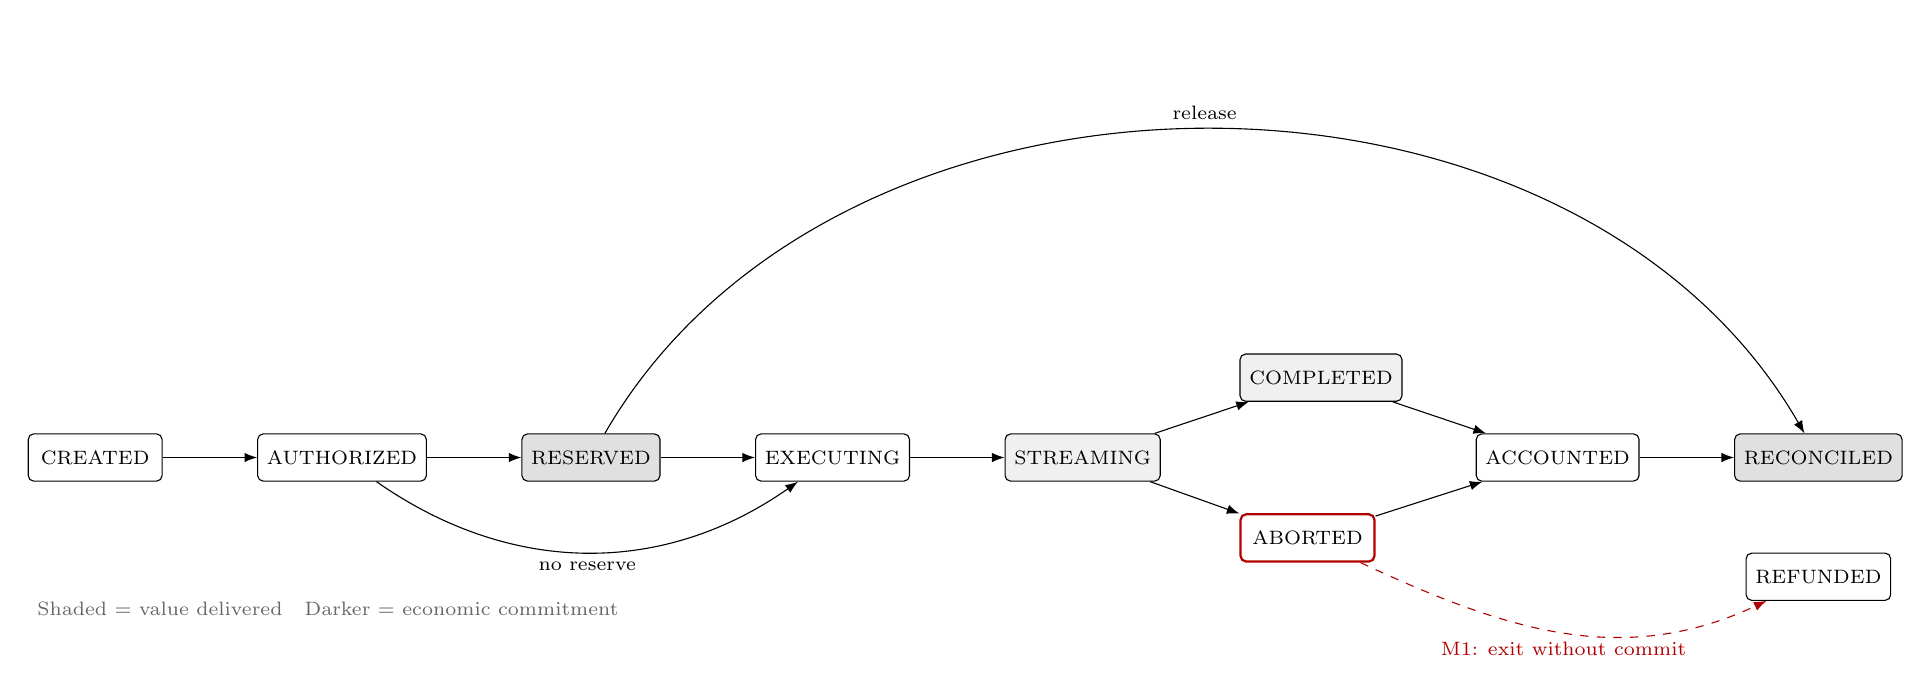
\begin{tikzpicture}[
  node distance=8mm and 12mm,
  every node/.style={font=\scriptsize},
  st/.style={draw, rounded corners=2pt, minimum height=6mm, minimum width=17mm, align=center},
  val/.style={st, fill=black!6},
  com/.style={st, fill=black!12},
  bad/.style={st, draw=red!70!black, thick},
  ->/.default=,
  arr/.style={-{Latex[length=1.6mm]}, thin},
  barr/.style={-{Latex[length=1.6mm]}, thin, red!70!black, dashed},
]
\node[st] (created) {CREATED};
\node[st, right=of created] (auth) {AUTHORIZED};
\node[com, right=of auth] (res) {RESERVED};
\node[st, right=of res] (exec) {EXECUTING};
\node[val, right=of exec] (stream) {STREAMING};
\node[val, above right=4mm and 10mm of stream] (comp) {COMPLETED};
\node[bad, below right=4mm and 10mm of stream] (abort) {ABORTED};
\node[st, right=14mm of stream, xshift=26mm] (acc) {ACCOUNTED};
\node[com, right=of acc] (rec) {RECONCILED};
\node[st, below=9mm of rec] (ref) {REFUNDED};
\draw[arr] (created) -- (auth);
\draw[arr] (auth) -- (res);
\draw[arr] (res) -- (exec);
\draw[arr] (auth) to[out=-35,in=-145] node[below,pos=.5]{no reserve} (exec);
\draw[arr] (exec) -- (stream);
\draw[arr] (stream) -- (comp);
\draw[arr] (stream) -- (abort);
\draw[arr] (comp) -- (acc);
\draw[arr] (abort) -- (acc);
\draw[arr] (acc) -- (rec);
\draw[barr] (abort) to[out=-25,in=-155] node[below,pos=.5]{\color{red!70!black}M1: exit without commit} (ref);
\draw[arr] (res) to[out=60,in=120] node[above,pos=.5]{release} (rec);
\node[align=left, anchor=north west] at ($(created.south west)+(0,-14mm)$) {%
  \color{black!60}Shaded = value delivered\quad Darker = economic commitment};
\end{tikzpicture}%
}
\caption{Request lifecycle. Value exposure begins at the first delivered token
(STREAMING); economic commitment is final only at RECONCILED. The interval between them
is the exposure window that M1 exploits. B0 corrupts the AUTHORIZED $\rightarrow$
RESERVED transition (non-atomic); M2 corrupts the data used at ACCOUNTED.}
\label{fig:statemachine}
\end{figure}

\subsection{Formal model}
For a request $r$ let $U_{\text{true}}(r)$ be the usage actually produced,
$U_{\text{bill}}(r)$ the usage billed, and $P(\cdot)$ the exact-decimal pricing function.
Write $C(r) = P(U_{\text{true}}(r))$ for the true cost, $V(r)$ for the value actually
delivered to the client, $\mathrm{Res}(r)$ for any reservation, $D(r)$ for committed
debits, $F(r)$ for refunds, and $N(r) = D(r) - F(r)$ for the net committed debit.
Under-payment and the integrity property are $\mathrm{Leak}(r) = V(r) - N(r)$ and
$\mathrm{Integrity}(r):\, V(r) \le N(r)$, as in Equation~(\ref{eq:integrity}). Because
legitimate reconciliation exists, integrity is an inequality on the net debit; a refund is
legitimate only when it releases the unconsumed portion, $F(r) \le \mathrm{Res}(r) -
V(r)$, as in Equation~(\ref{eq:refund}). At trial level the harness independently verifies
conservation, $\sum_{r \in T} N(r) = B_{\text{initial}} - B_{\text{final}}$, and fails the
build on any divergence.

\subsection{Mechanism localization}
\paragraph{B0 (synchronization).}
The baseline implementation manifests as follows: if two concurrent requests read the
same authorization state $B$ and both commit a decrement derived from it, one decrement
is lost, $\sum_i N(r_i) < \sum_i V(r_i)$. This particular manifestation requires two or
more overlapping transactions, which is why the baseline leaks nothing at concurrency 1.
The general failure condition is broader than this trigger, however: the defect occurs
whenever authorization observes a state that does not yet reflect the economic
commitments generated by other authorized requests. Concurrent overlap is one way to
create that condition; Section~\ref{sec:b0revised} shows that deferred settlement creates
the same condition under strictly sequential arrivals, with no overlap at all. We
therefore distinguish, throughout this paper, the \emph{baseline trigger} (concurrent
overlap, in this implementation) from the \emph{general security condition}
(authorization not atomically coupled to economic commitment on the authorizing path).

\paragraph{M1 (commitment timing).}
If $V(r) > 0$ in STREAMING but the exit path taken (ABORTED) does not reach RECONCILED
with $N(r) \ge V(r)$, then $\mathrm{Leak}(r) = V(r) > 0$. The defect is in the transition
graph, not in a shared resource: it is a per-request lifecycle property, and
Section~\ref{sec:m1} confirms empirically that it does not depend on concurrency in the
tested architecture.

\paragraph{M2 (usage authority).}
If the billing basis is client-controlled, $U_{\text{bill}} = T(U_{\text{true}})$ for an
attacker transformation $T$, then $\mathrm{Leak}(r) = P(U_{\text{true}}) -
P(T(U_{\text{true}})) > 0$ whenever $P \circ T < P$. Authority is a per-request
data-provenance property; Section~\ref{sec:m2} shows this is analytically independent of
concurrency because the billed amount never reads shared mutable state.

\begin{table}[t]
\centering
\caption{Structural distinction between the three mechanisms: what is defective, what
triggers the baseline manifestation we implemented, and what closes it. ``Trigger'' is
implementation-specific; the general condition (final column of Table~\ref{tab:practical})
is what actually matters and is not concurrency-specific for any of the three.}
\label{tab:structural}
\resizebox{\linewidth}{!}{%
\begin{tabular}{llll}
\toprule
Mechanism & Defective element & Baseline trigger (this implementation) & Closed by \\
\midrule
B0 & transition atomicity & overlapping requests (concurrency $\ge 2$); deferred settlement also suffices (Sec.~\ref{sec:b0revised}) & authorization atomically coupled to commitment on the authorizing path \\
M1 & transition graph (abort path) & any single abort, no concurrency needed & abort-inclusive finalization \\
M2 & data authority at ACCOUNTED & any single request with a client-controlled billing basis, no concurrency needed & server-authoritative recount \\
\bottomrule
\end{tabular}%
}
\end{table}

This predicts the empirical result of Section~\ref{sec:results}: the baseline B0
manifestation we implemented is created by concurrency, while M1 and M2 per-request
leakage is invariant to it in the tested design --- and Section~\ref{sec:generality}
shows the B0 baseline's concurrency dependence was a property of that one trigger, not
of the underlying failure condition.

\section{Architectural Taxonomy}
\label{sec:taxonomy}
The three dimensions are experimentally distinguishable rather than merely conceptual. B0
is a non-atomic authorize-then-decrement on shared credit state; it is a known baseline,
used to validate the measurement rig and to supply a generic reference point. M1 is
lifecycle-sensitive: it concerns which terminal paths reach a committed accounting event.
M2 is authority- and pricing-sensitive: it concerns which representation of usage the
billing function actually reads.

\subsection{On LLM specificity}
We do not claim these mechanisms are possible only in LLM systems. Streaming responses,
trusting client-supplied values, and racing a counter all occur elsewhere. What is
specific to LLM inference is that one request combines, at a single metering boundary:
progressive value delivery; usage that is generated at runtime and therefore unknown at
authorization time; multi-category token vectors; tokenizer- and provider-dependent usage
semantics; pricing functions defined over those categories; and asynchronous settlement.
It is the combination we systematize, not the individual pieces.

On that basis B0 remains generic --- a shared-counter race that behaves the same in any
metered API --- while M1 and M2 are LLM-relevant accounting dimensions. M1 is only
interesting where value is delivered progressively over a long-running request, and M2
only where the billed quantity is a runtime-produced, multi-category vector priced by a
category-sensitive function. The security subject throughout this paper is the metering
and accounting infrastructure around inference, not the behavior, robustness, or output
safety of the language model itself.

\section{System and Experimental Methodology}
\label{sec:method}
The testbed is a FastAPI gateway over PostgreSQL 16 in READ COMMITTED and Redis 7,
running under Docker Compose on one commodity host with 16 logical CPUs and 16\,GB of
RAM. Money is exact decimal throughout. Five M1 architectures and six M2 architectures
sit behind common interfaces, so experiments compare semantics rather than unrelated
code. The default generator is deterministic, which is what makes the accounting
arithmetic exact; real tokenizers run on the recount path, and
Section~\ref{sec:generality} replaces the generator entirely with third-party serving
code.

Pricing is category-wise over three tiers. Leakage \emph{efficiency} --- the fraction of
true value evaded --- is the headline metric because it is invariant under uniform price
scaling; absolute dollar figures are labeled as scenario values. The sweeps are: B0
concurrency $\{1,2,5,10,20,30,50\}$ with 30 repetitions; M1 across architecture, abort
position, and concurrency $\{1,5,20,50,100\}$; M2 across architecture, manipulation, and
concurrency. Request volume is held constant across concurrency levels, so that volume
cannot masquerade as vulnerability.

\subsection{Integrity gates}
Every summarizer recomputes each record's leak from primitives, checks invariant-flag
consistency, and verifies ledger conservation $\sum_r N(r) = B_{\mathrm{init}} -
B_{\mathrm{final}}$ without trusting the application's own bookkeeping. A violation fails
the build. The gates are validated adversarially rather than assumed: corrupting a leak
value, a debit, a served flag, a balance, or an invariant flag, and deleting a ledger row,
must each be detected, and all twelve injections were. The metamorphic suite also caught
one of our own unjustified assumptions. We had asserted that leakage efficiency is
invariant across price tiers; it is, but only under uniform scaling, not under a
structural change to the price ratios. We corrected the property rather than suppress the
failure.

\subsection{Independent verification}
The strongest M2 defense is re-implemented in a module that shares no code path with the
gateway, and the two agree on all cross-validated cells (42 M2, 16 M1, 2 B0). A separate
audit re-derives every reported quantity from raw data using code that imports nothing
from the project, and reports zero discrepancies across 4{,}800 M2 records, 2{,}400 M1
records, and 420 B0 trials. The independent checker initially reported three
disagreements. They were definitional rather than defects: the checker aggregated
under-payment only, while the gateway aggregates the signed billing delta, and under
flat-total pricing an honest client is systematically overcharged, so the two aggregates
legitimately differ. Both are now reported, and the security property uses under-payment.

\subsection{Statistics}
All statistics come from a standalone script using SciPy and statsmodels, writing a
single output file that the paper cites. Many conditions here are deterministic by
construction and have exactly zero variance. For those we report the constant and the
complete separation rather than a $p$-value, and reserve nonparametric tests and
bootstrap intervals for quantities that genuinely vary.

\section{Formal Verification}
\label{sec:formal}
Measurement shows that a defect occurs on the schedules our harness produced. It cannot
show that a defended architecture is safe on schedules it did not produce. We therefore
encode the lifecycle of Section~\ref{sec:statemodel} in TLA+ \citep{tla} and check it
exhaustively with TLC 2.19 \citep{tlc}.

\subsection{Model}
One specification covers all three dimensions, with each dimension as a Boolean constant,
so that the safe and unsafe architectures are the same state machine under different
constants --- exactly how the testbed implements them behind one interface. The constants
are \texttt{AtomicDebit} for B0, \texttt{Reserves} and \texttt{AbortSafe} for M1, and
\texttt{ServerAuthority} for M2. A fifth constant, \texttt{ClientMayAbort}, is a workload
switch rather than an architecture property; disabling it in the B0 configurations keeps
the synchronization counterexample free of commitment-timing noise, mirroring how the
experiments hold the other dimensions at their safe setting.

Four invariants are checked, each the formal counterpart of a gate the summarizers
already apply to every record: \textsc{AccountingIntegrity} ($V(r) \le N(r)$ for terminal
$r$), \textsc{Solvency} ($\mathrm{balance} \ge 0$), \textsc{LedgerConservation} (once all
requests are terminal, $B_{\mathrm{init}} - B_{\mathrm{final}} = \sum_r N(r)$), and
\textsc{RefundBounded}, which is Equation~(\ref{eq:refund}). Solvency is checked
separately from accounting integrity; collapsing them would destroy the distinction the
ablation exists to establish.

\subsection{Method}
Each invariant is checked in its own TLC run. TLC halts at the first violation it finds,
so checking jointly would hide the fact that an M2 architecture breaks two of them. The
result is a full configuration $\times$ invariant matrix (Table~\ref{tab:formalmatrix}):
ten configurations and four invariants give 40 independent runs over 27{,}526 distinct
states. Every expected outcome is declared in the checking script before the run, and the
script exits non-zero on any disagreement. All 40 matched, with no disagreements. Runs
use a single worker deliberately: with parallel workers, a run that halts at a
counterexample explores a nondeterministic number of states, and the totals drifted
between runs.

\begin{table}[t]
\centering
\caption{TLC model-checking results across ten architecture configurations and four
invariants. All 40 outcomes matched the expectation declared before the run.}
\label{tab:formalmatrix}
\resizebox{\linewidth}{!}{%
\begin{tabular}{lllll}
\toprule
Configuration & Accounting integrity & Solvency & Ledger conservation & Refund bounded \\
\midrule
b0 vulnerable & holds & holds & VIOLATED & holds \\
b0 hardened & holds & holds & holds & holds \\
m1 post completion & VIOLATED & holds & holds & holds \\
m1 reserve refund on abort & VIOLATED & holds & holds & VIOLATED \\
m1 no reserve settle & holds & VIOLATED & holds & holds \\
m1 reserve reconcile & holds & holds & holds & holds \\
m2 client & VIOLATED & holds & holds & VIOLATED \\
m2 server recount & holds & holds & holds & holds \\
all defenses & holds & holds & holds & holds \\
all defenses 3req & holds & holds & holds & holds \\
\bottomrule
\end{tabular}}
\end{table}

\subsection{Counterexamples}
TLC returns a shortest counterexample for each unsafe configuration, and each reproduces
the mechanism we measured. For B0, the 21-step trace is the lost update exactly: both
requests read the same balance, both write an absolute value derived from that stale
read, and both then deliver and are charged. Which invariant fails is the interesting
part. Accounting integrity and the refund bound both hold, because every individual
record is internally consistent; what breaks is conservation of the shared balance. That
is why a per-record audit cannot detect B0 while a conservation check can.

For M1, the model checks all four combinations of reservation and abort-safe
finalization, not just the two the implementation ships. Reservation alone yields
solvency and violates integrity. Abort-safe finalization alone yields integrity and
drives the balance to $-1$. Only the conjunction satisfies both. The orthogonality claim
is therefore established by exhaustive exploration rather than by the two architectures
we happened to build.

For M2, the client-authoritative architecture violates accounting integrity and also the
refund bound: with a reservation in place, under-billing surfaces as an over-refund. That
the same defect appears in two independent invariants is a consequence of the model
rather than something we set out to show, and it became visible only because the
invariants are checked separately. Enabling server authority restores all four invariants
against the same lying client; the declared value simply stops being read.

The three defenses also compose. With contention, aborts, and a lying client all enabled,
no invariant is violated on any reachable state, at two and at three concurrent requests.

\subsection{Evidence labels and their limits}
We use three labels and do not interchange them. \emph{Model-checked} means TLC explored
the reachable state space exhaustively under a stated configuration. \emph{Formally
argued} means stated over the accounting model and reasoned about by hand.
\emph{Empirically verified} means measured and independently recomputed. Nothing weaker
than the first is ever described as proved.

Nothing here shows that a production implementation is safe. The model abstracts away
the database, the network, partial failure, asynchronous reconciliation, multi-category
pricing, and tokenizer disagreement. It is finite, at two to three requests with unit
pricing. Only safety properties are checked; no liveness property is verified. \textbf{We
do not provide a mechanized refinement proof from the abstract specification to the
implementation.} The correspondence between the two is an argument supported by
case-by-case agreement between formal and empirical outcomes, and we do not claim more.

\subsection{The specification was wrong first}
Declaring expectations before running earned its keep immediately. Our first
specification treated a reservation as a hold and set the committed debit equal to the
charge at settlement, so $N = D - F$ fell below the delivered value and TLC rejected the
safe configurations. The model was wrong, not the paper: in a reserve-and-reconcile
architecture the reservation \emph{is} the committed debit, and the refund returns its
unused part. Correcting the settlement semantics made the safe configurations verify. We
record the failure because a formal model that is edited until it agrees with the paper
is worth nothing.

\section{Empirical Results}
\label{sec:results}

\subsection{B0: synchronization}
The non-atomic check-then-decrement baseline leaks only when at least two requests
overlap; this is a property of the implemented trigger, and Section~\ref{sec:b0revised}
shows a different trigger for the same underlying condition. Mean leakage is \$0.000 at
concurrency 1, then \$0.099, \$2.871, and \$4.851 at concurrency 2, 30, and 50, growing
linearly at 0.099 per additional concurrent request with $R^2 = 1.0000$ and $p = 1.9
\times 10^{-50}$ (Figure~\ref{fig:b0}). The hardened atomic compare-and-decrement leaks
nothing at every level.
B0 is not a contribution; it validates the rig and supplies the contrast used below.
Section~\ref{sec:generality} revises the conclusion drawn from it.

\begin{figure}[t]
\centering
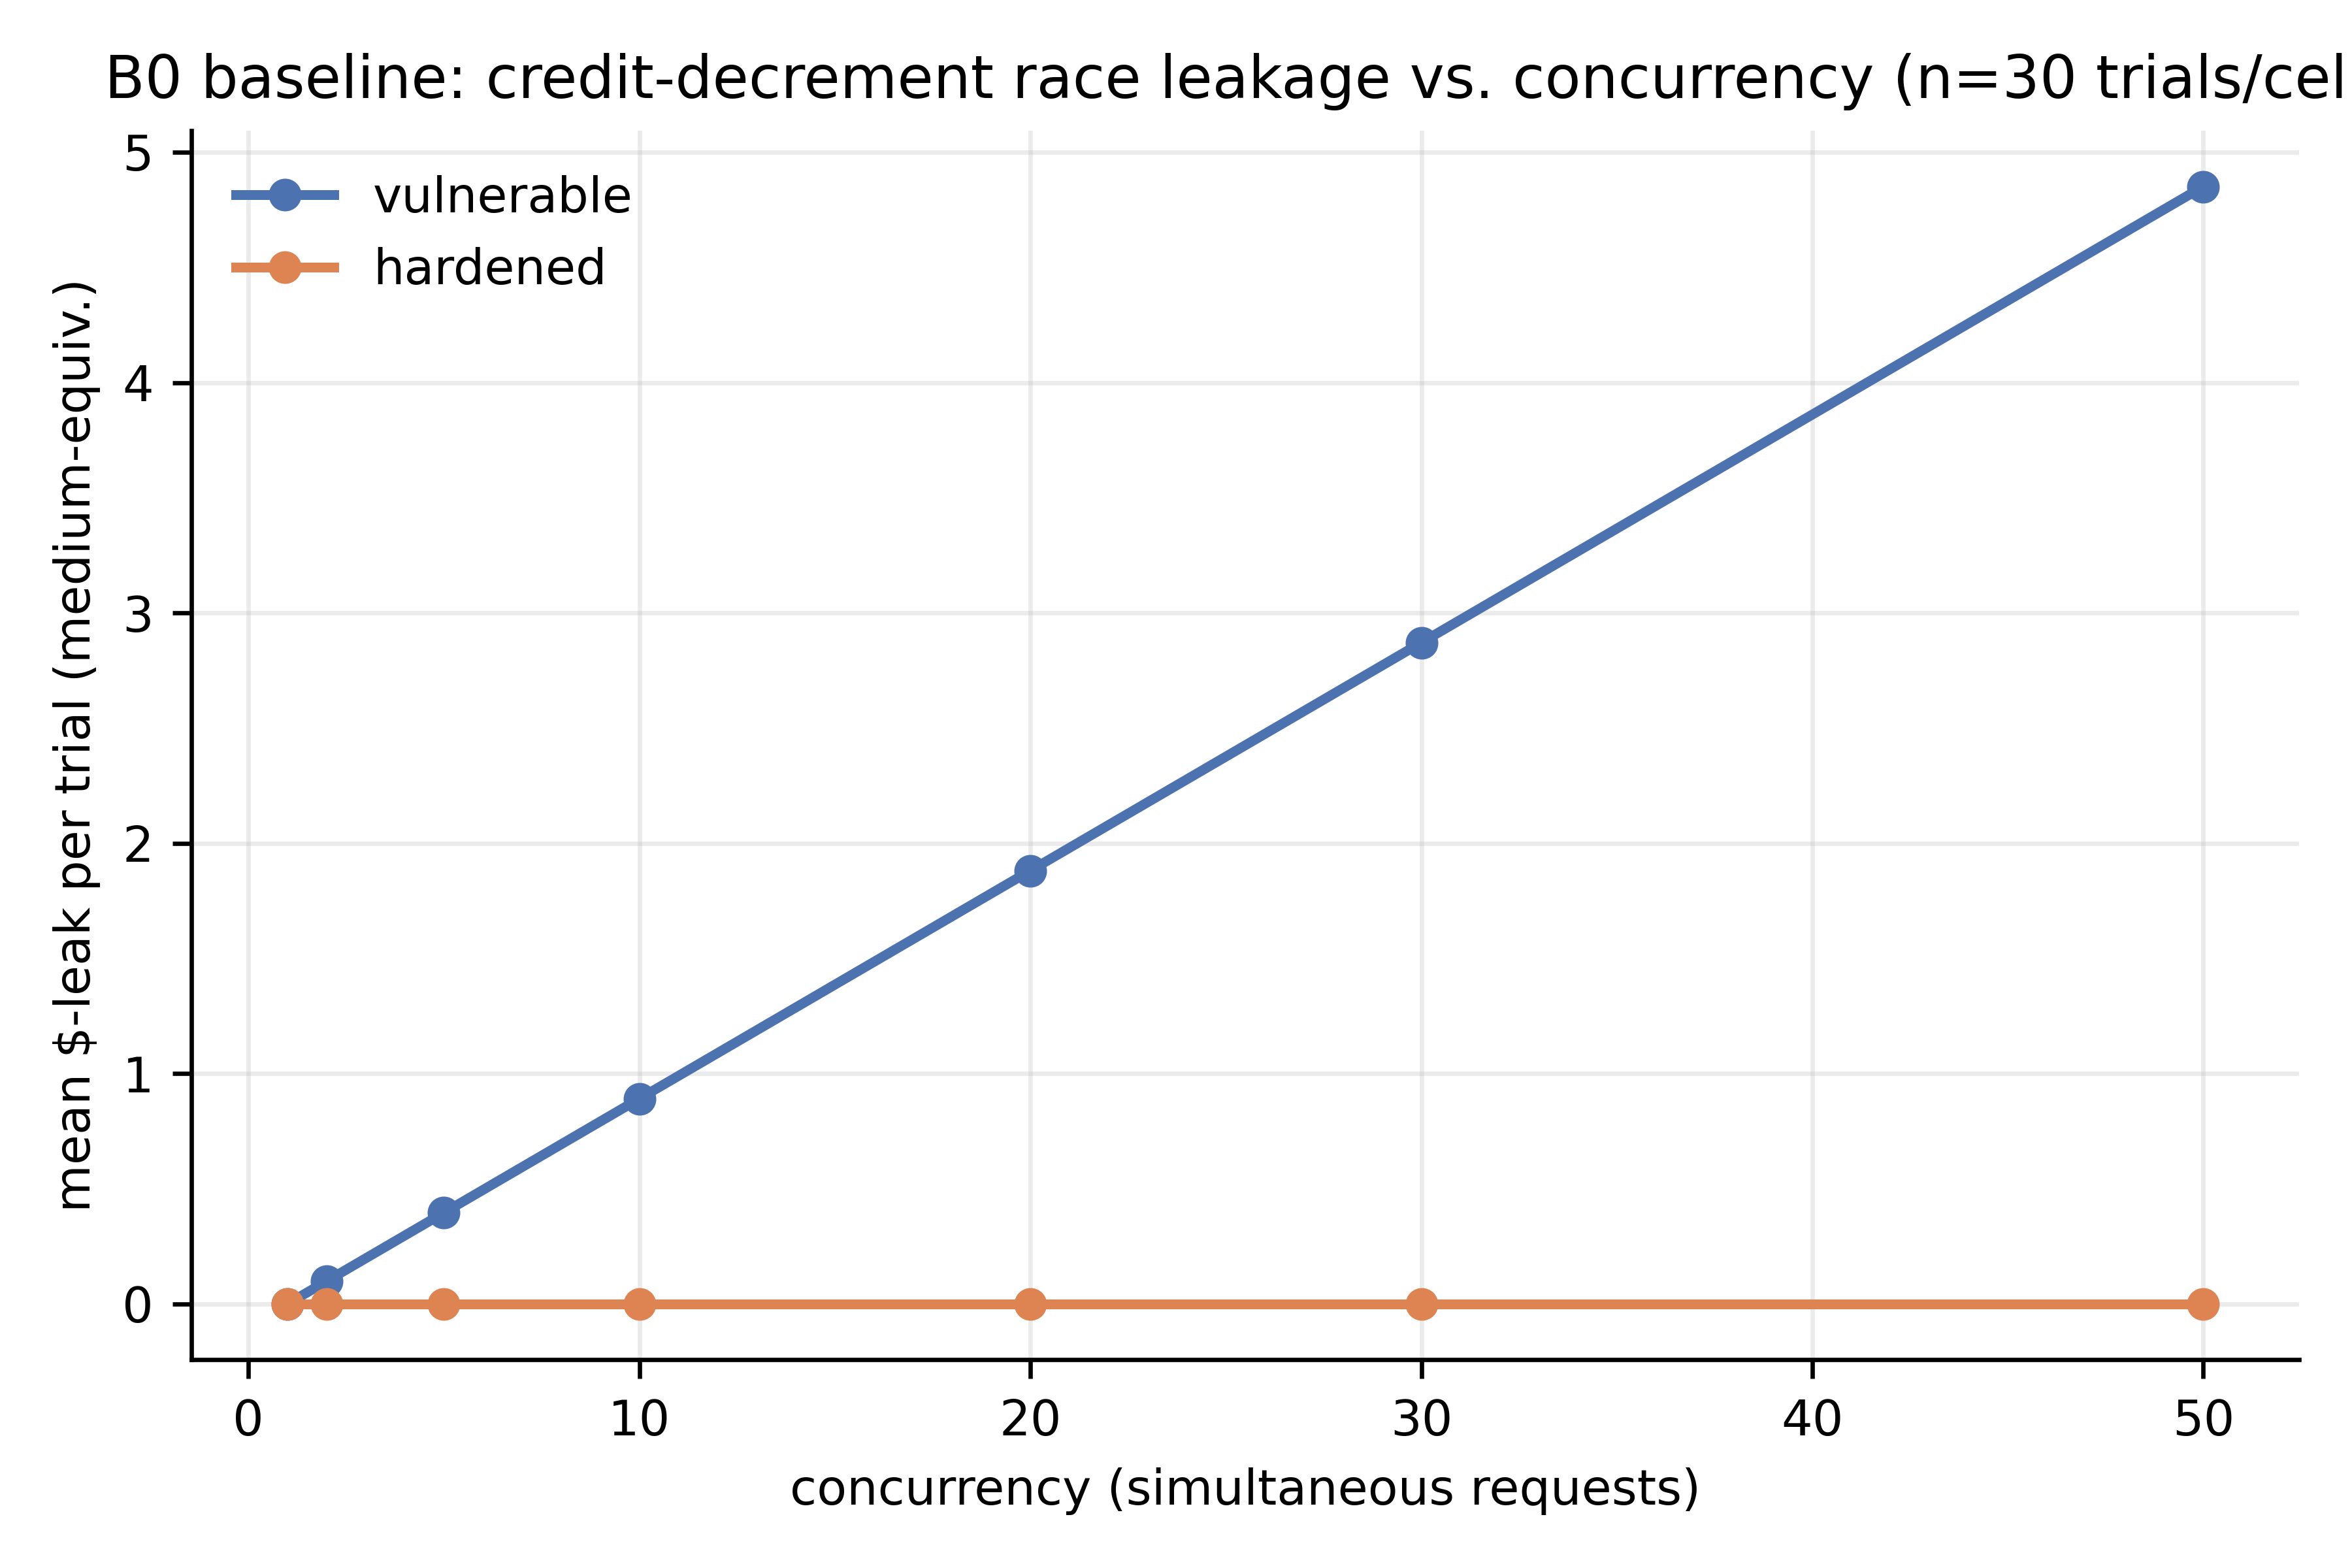
\includegraphics[width=\linewidth]{Figure_2.png}
\caption{B0 baseline: mean leakage per trial against concurrency, 30 repetitions per
cell, deterministic generator. Leakage is created by contention in this baseline
implementation, growing linearly at 0.099 per additional concurrent request ($R^2 =
1.0000$). Section~\ref{sec:b0revised} shows that concurrency is not the essential
ingredient in the general condition: delayed settlement produces the same over-serving
with strictly sequential arrivals.}
\label{fig:b0}
\end{figure}

\subsection{M1: commitment timing}
\label{sec:m1}
Leakage tracks the value delivered before the missing commit. It rises monotonically
with abort position and collapses to zero at completion, when the debit finally fires:
per request, \$0.0045 at roughly one token delivered, \$0.0285 at 25\%, \$0.0540 at 50\%,
\$0.0960 at 90\%, and \$0.0000 at completion (Figure~\ref{fig:m1}). Request-level attack
success is 1.00 at every abort position before completion. The two vulnerable
architectures --- debit only after completion, and refund the whole reservation on abort
--- are economically identical.

\begin{figure}[t]
\centering
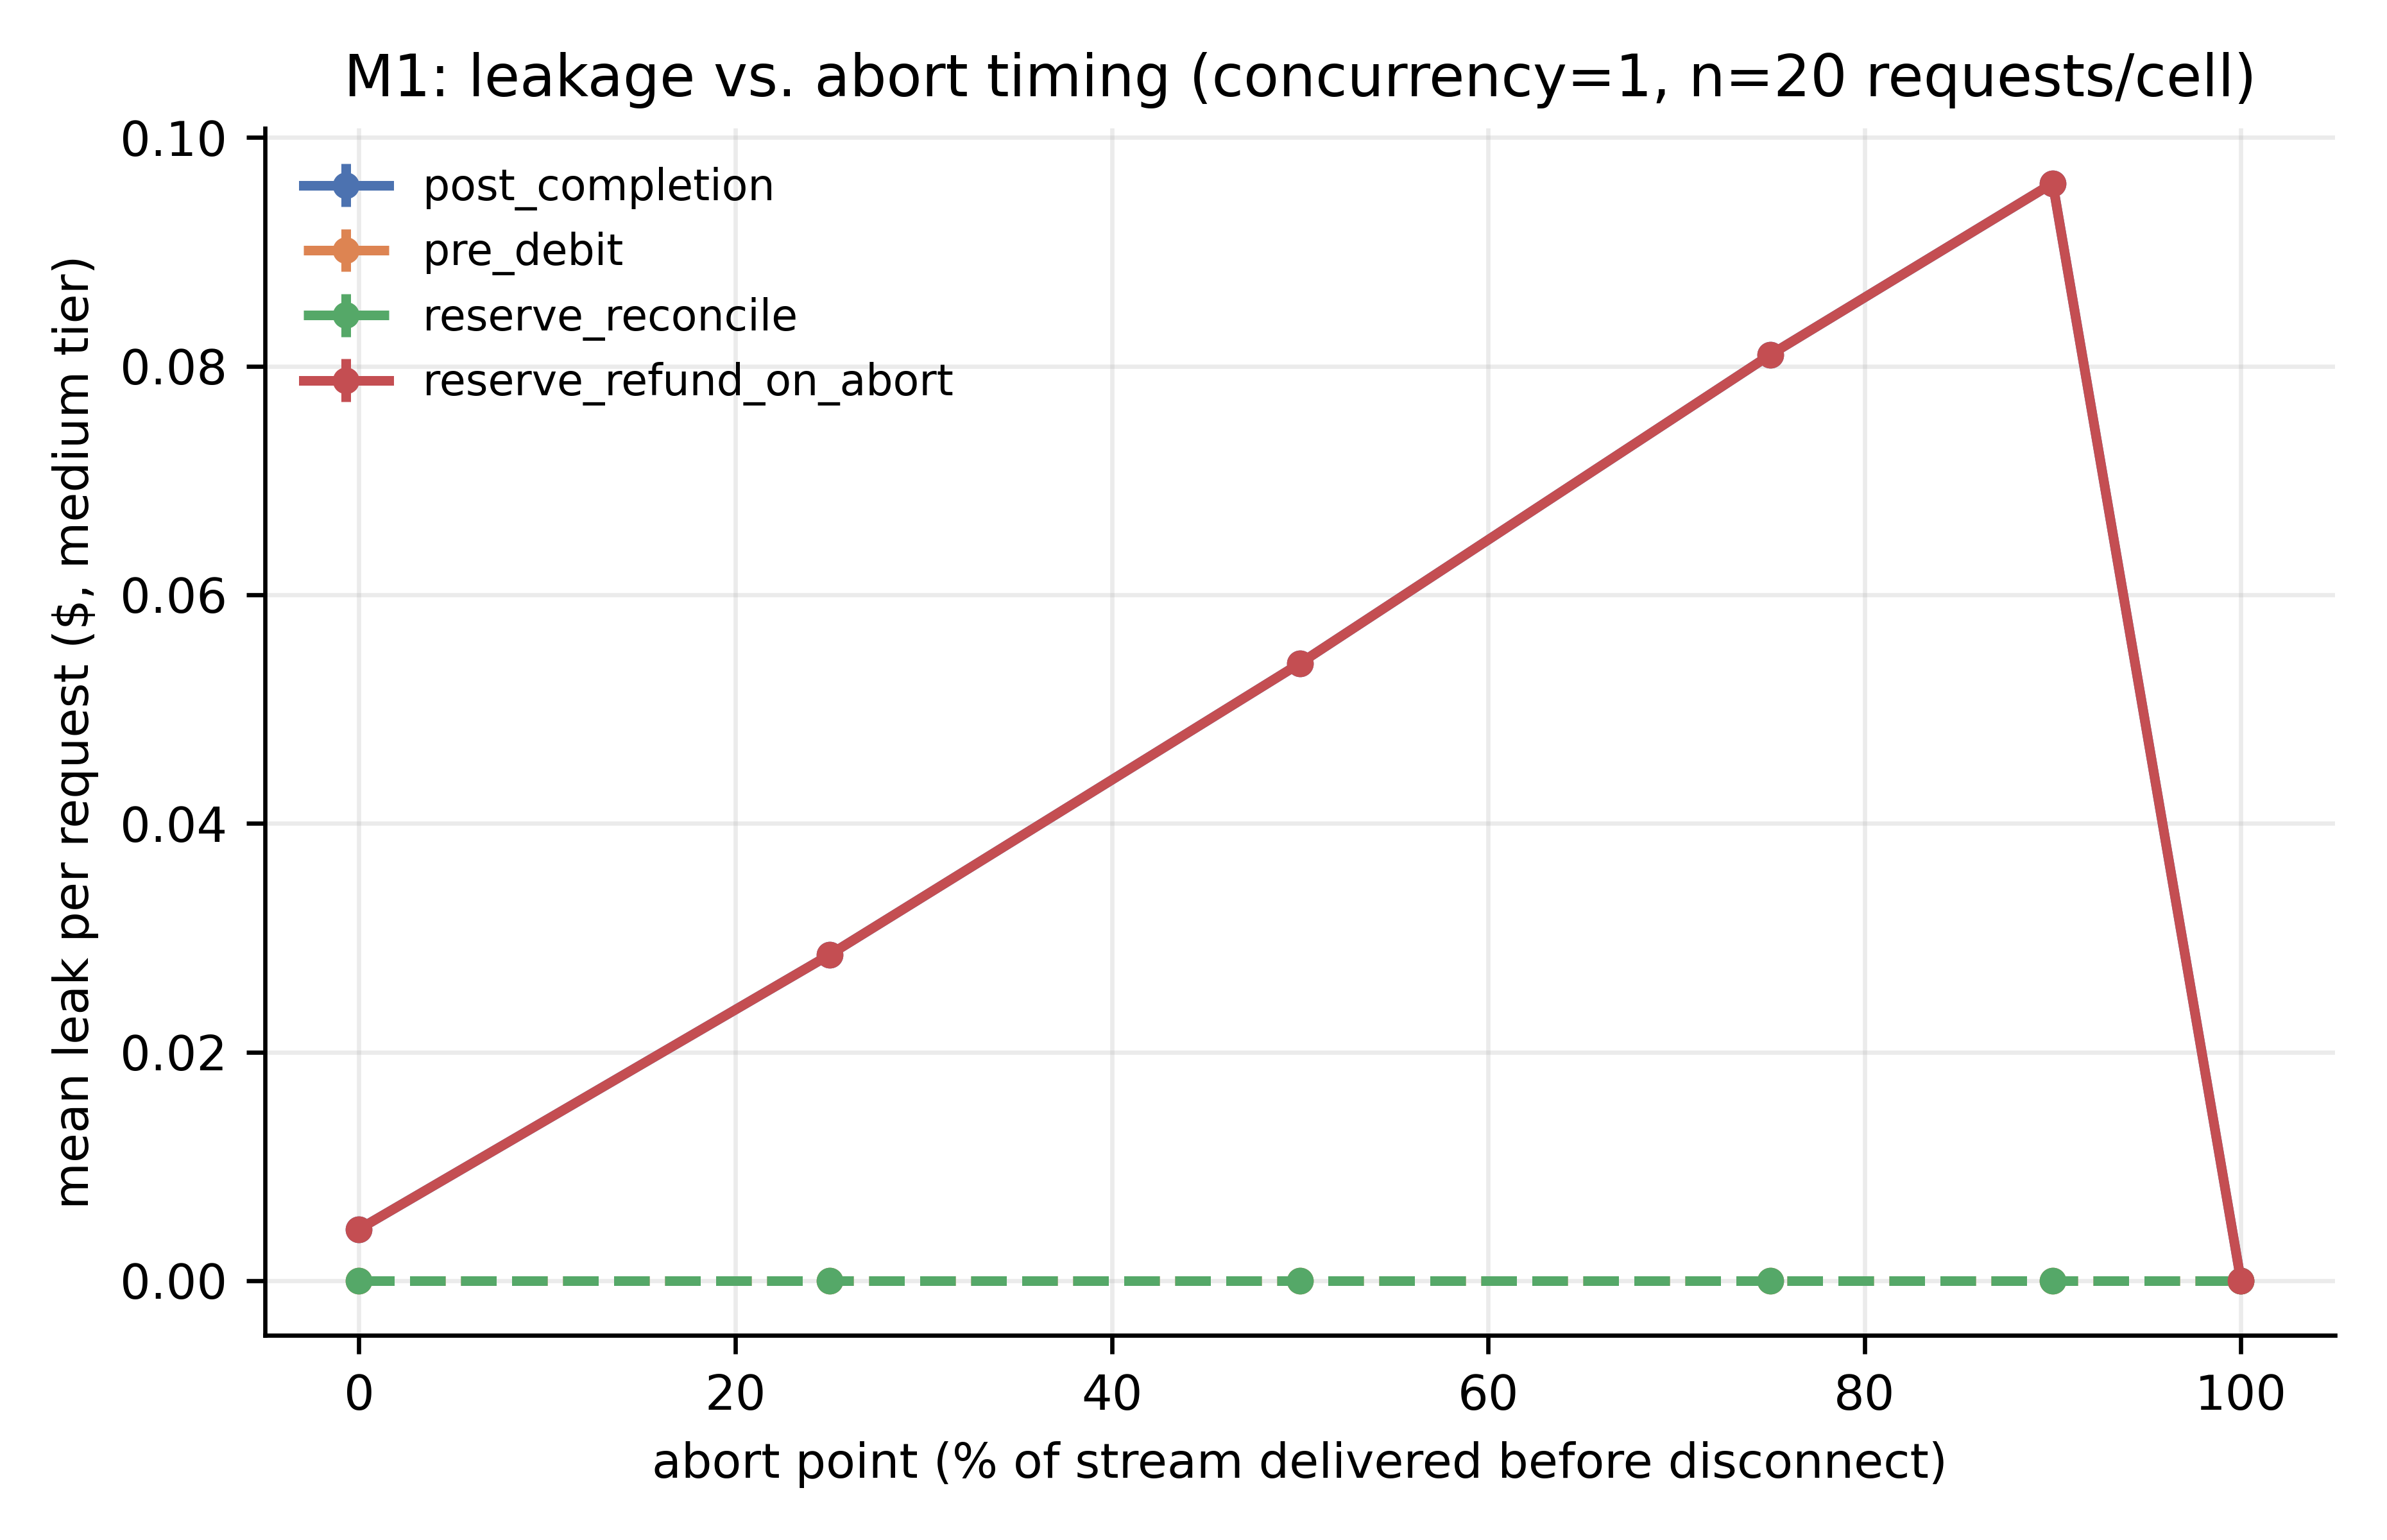
\includegraphics[width=\linewidth]{Figure_3.png}
\caption{M1 leakage against abort position, deterministic generator, concurrency 1,
medium price tier, 20 requests per cell. The $x$-axis is the fraction of the response
streamed before the client disconnects; the $y$-axis is mean leakage per request in
scenario dollars, i.e., delivered value minus net committed debit. Vulnerable
architectures peak just before the commit would have fired and collapse to \$0 at
completion, when it does fire; safe architectures stay at \$0 throughout. All values are
empirical. Error bars are within-cell standard deviations and are zero at this
concurrency.}
\label{fig:m1}
\end{figure}

\subsubsection{Two orthogonal properties}
The ablation separates solvency from accounting finality. Given a budget for two requests
and six issued, the no-reserve-settle architecture preserves accounting integrity ---
leakage is \$0.0000 at every abort position --- yet serves all six and drives the balance
to $-\$0.32$. Conversely, the reserve-refund-on-abort architecture holds a reservation
and then refunds it away, failing both. Table~\ref{tab:m1orth} states the resulting
design rule; Section~\ref{sec:formal} establishes it exhaustively rather than by these
two examples.

\begin{table}[t]
\caption{M1 orthogonality. Each control secures one property; only the conjunction
secures both. All four cells are model-checked (Table~\ref{tab:formalmatrix}); the
diagonal cells are also measured.}
\label{tab:m1orth}
\centering
\begin{tabular}{lll}
\toprule
 & \multicolumn{2}{c}{Reservation} \\
\cmidrule(l){2-3}
Abort-safe finalization & No & Yes \\
\midrule
No & neither property & solvency only \\
Yes & integrity only & both \\
\bottomrule
\end{tabular}
\end{table}

\begin{figure}[t]
\centering
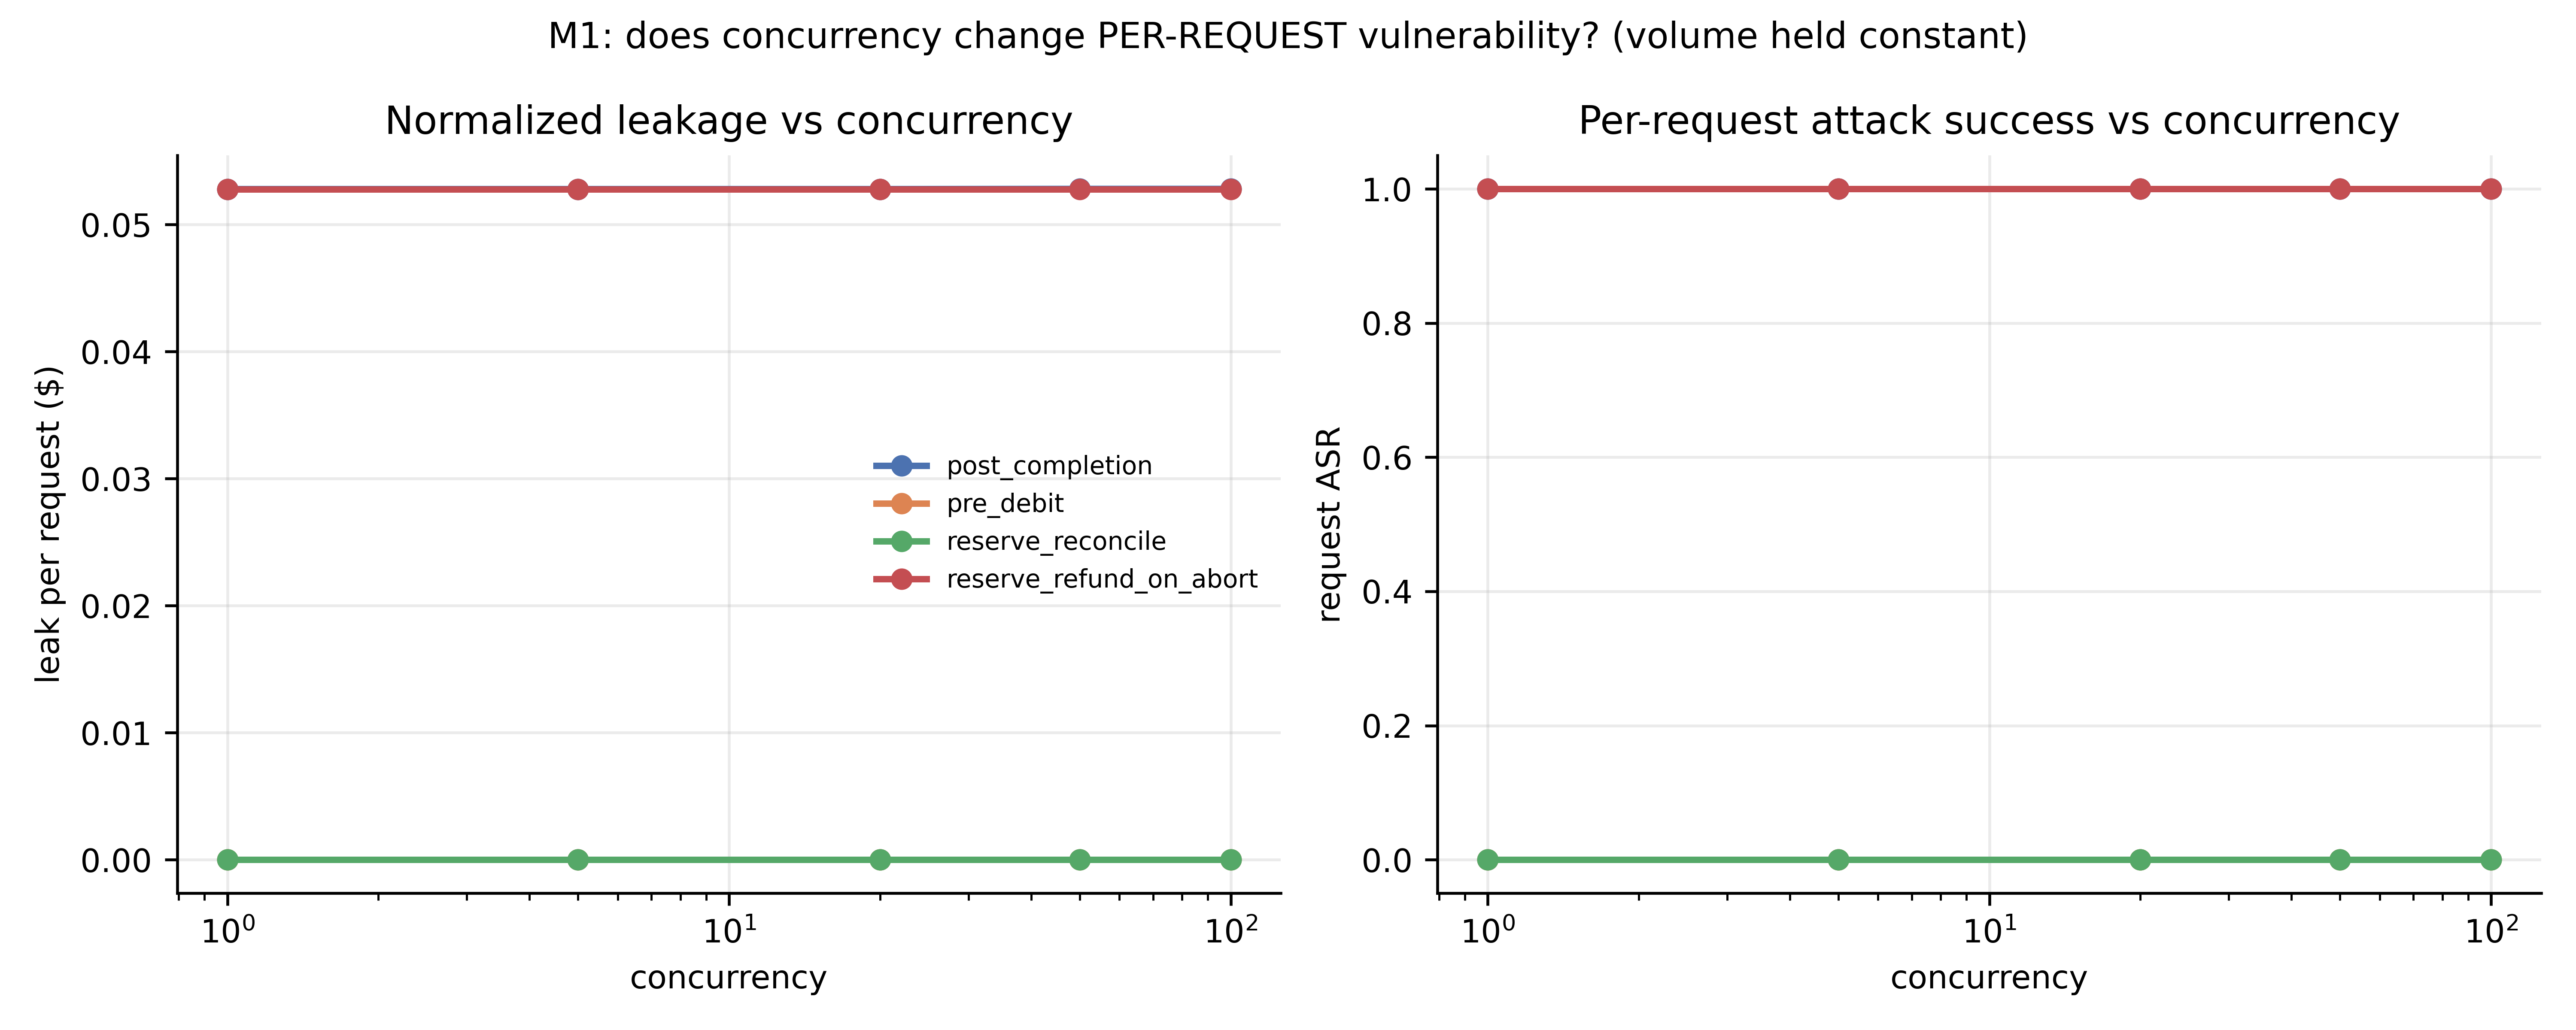
\includegraphics[width=\linewidth]{Figure_4.png}
\caption{M1 negative result. Request volume is held constant at 20 requests per cell
while concurrency varies from 1 to 100 ($x$-axis, log scale); the $y$-axis is mean
leakage per request and request-level attack success. Both are invariant across the
range, which is the empirical basis for treating commitment timing as a per-request
rather than a contention-driven defect. Holding volume constant is what prevents traffic
level from masquerading as vulnerability.}
\label{fig:m1conc}
\end{figure}

\subsubsection{Concurrency is not the mechanism}
With request volume held constant, per-request leakage was unchanged across concurrency
levels 1 to 100: \$0.0528 per request at every level, identical to four decimal places,
with request-level attack success exactly 1.000 for vulnerable and 0.000 for safe
architectures (Figure~\ref{fig:m1conc}). The honest-client control leaked nothing
anywhere. We do not claim
invariance as a proven property of all systems under all loads; this is the measured
behavior of the tested architecture, and Section~\ref{sec:discussion} gives the
structural reason the model predicts it.

\subsection{M2: usage authority}
\label{sec:m2}
The M2 result is best read as a chain. True usage is produced by the model; usage
computation turns it into a vector; that vector is stored; a billing authority decides
which representation to price; and a debit follows. A system can compute and store the
correct usage while still billing from a different, attacker-influenced representation,
and nothing in the chain flags the discrepancy.

That is not hypothetical. The client-logged architecture performs an accurate
server-side recount, records it alongside the declared vector, and bills the declared
number. Against 90\% output under-reporting it leaks 58.3\% of delivered value in the
controlled setting, and 69.0\% against the real serving stack of
Section~\ref{sec:generality}. The manipulation is K0: a client can count the tokens it
received, so no privileged knowledge is required. Every server-authoritative
architecture --- server-recount, hybrid-reconcile, and upstream --- drove leakage
efficiency to 0.000 across all eight manipulations in the tested catalog
(Figure~\ref{fig:m2}).

Writing $U$ for the true usage vector, $P$ for the pricing function, and $T$ for the
attacker's transformation of declared usage, a manipulation pays off exactly when
\begin{equation}
P(T(U)) < P(U),
\label{eq:m2}
\end{equation}
that is, when the pricing basis reads the field $T$ changes. Section~\ref{sec:economics}
develops the consequences. The exploitable set is a property of the billing function, not
of attacker ingenuity.

M2's independence from concurrency is analytic rather than discovered. The billed amount
is a pure function of one request's declared usage, computed before any balance is read,
so no shared mutable state enters the billing decision and the leak of one request cannot
depend on what else is in flight. The concurrency sweep confirms the derivation and
serves as a check that the implementation contains no unintended shared-state dependency.
It passes, and we present it as a much weaker claim than B0's measured slope.

\begin{figure}[t]
\centering
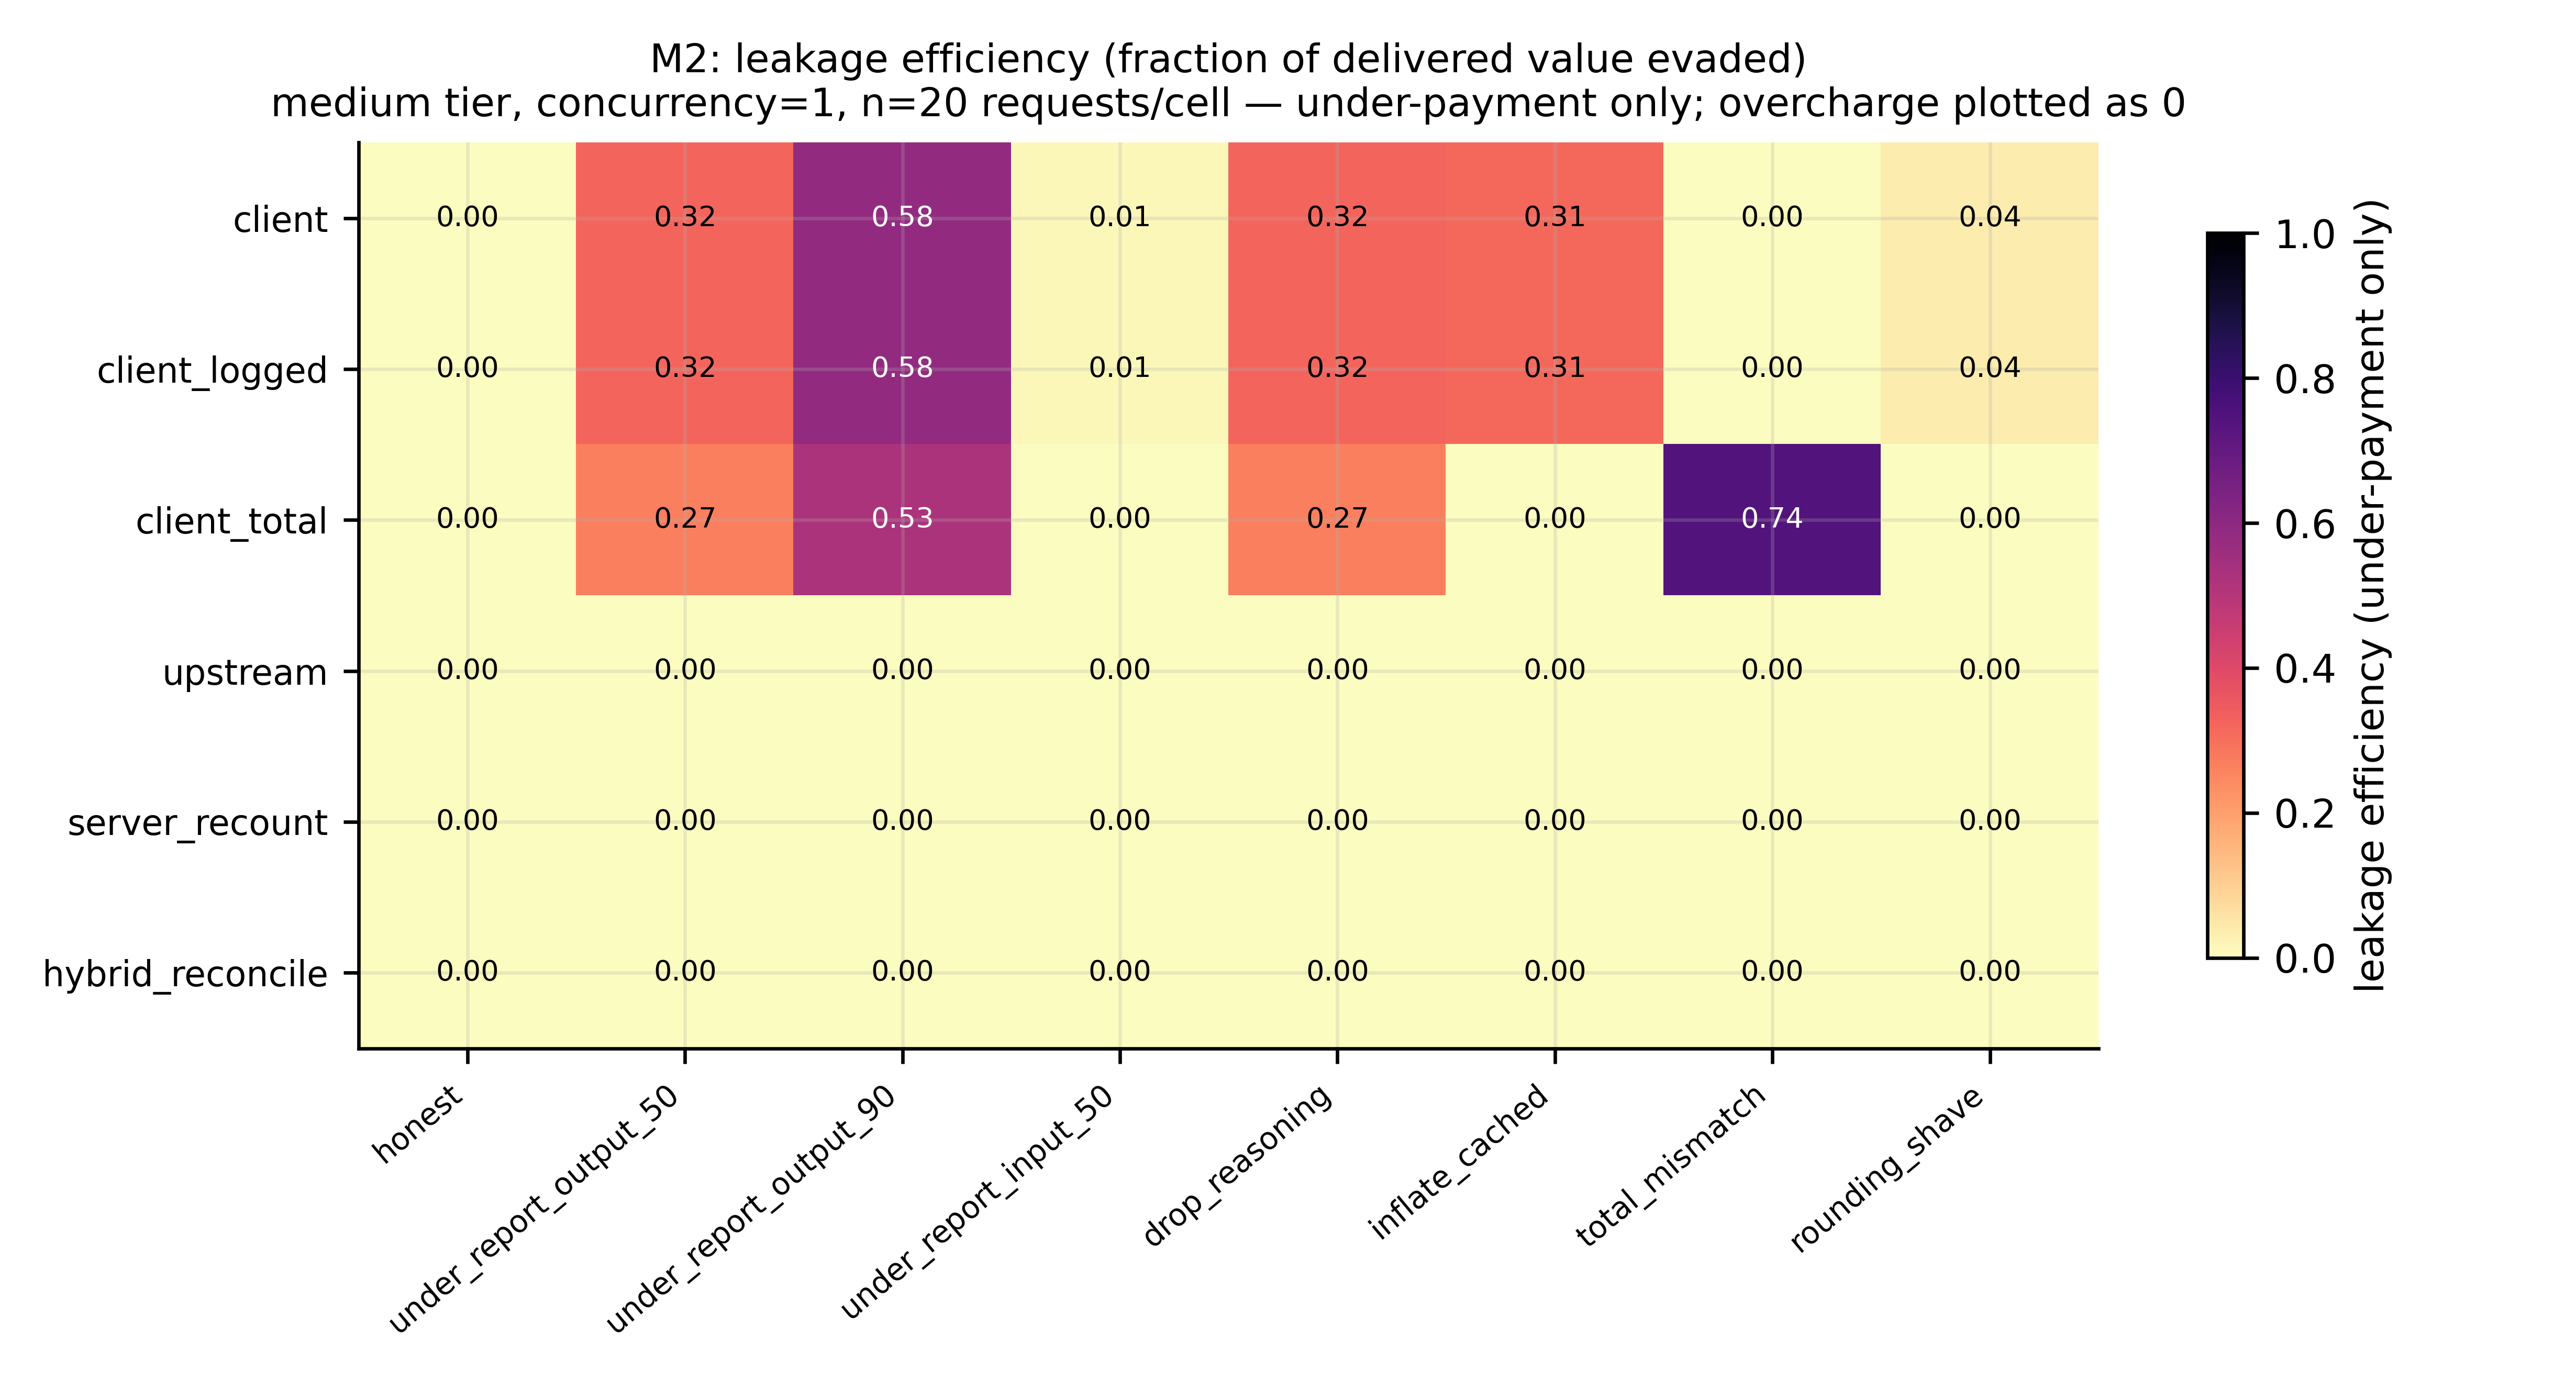
\includegraphics[width=\linewidth]{Figure_5.png}
\caption{M2 leakage efficiency --- the fraction of delivered value evaded --- by
architecture (rows) against declared-usage manipulation (columns), deterministic
generator, medium tier, concurrency 1, 100 requests per cell. Server-authoritative rows
are uniformly zero. The exploitable set differs between category-additive and flat-total
pricing, which is the empirical form of Equation~(\ref{eq:m2}): a manipulation pays off
only when the pricing basis reads the field it changes.}
\label{fig:m2}
\end{figure}

\subsection{Lifecycle failure modes}
Beyond the scripted attacks we inject nine lifecycle failures: disconnect at $t=0$ and
mid-stream, truncated stream, settle-window race, missing, delayed, and duplicated usage
metadata, and a recount-engine failure. Every invariant violation falls on a vulnerable
architecture, the hardened architectures survive all of them, and a recount-engine
failure is fail-closed --- the request is rejected and nothing is served or billed.

\subsection{A withdrawn claim}
\label{sec:detect}
An earlier version of this work reported a detectability taxonomy and claimed that
logging a server-side recount moved a leak from invisible to post-hoc reconcilable. An
independent audit of our own artifact showed the claim was not supported, and we
withdraw it.

Two defects were involved. The implementation assigned the detectability level from
static architecture metadata rather than measuring it, so the experiment read back a
label we had set. When we replaced that with a classifier reading only retained ledger
evidence and blind to architecture labels, the distinction disappeared: the two
architectures in question retain identical evidence, so both are equally reconcilable.
Across the full dataset, 2{,}200 records carrying the stored ``invisible'' label are
reconcilable or prevented on the evidence, and no record in the study qualifies as
invisible at all.

The root cause is a property of the testbed rather than of the architectures: our
harness records ground-truth usage for every architecture because it needs that value to
compute leakage, whereas a production deployment need not retain it. Our instrumentation
therefore cannot distinguish detectability classes, so we make no detectability claim. We
report this as a limitation rather than build additional instrumentation to rescue the
metric.

\section{Defenses and Sufficiency Conditions}
\label{sec:sufficiency}
The ablation shows which primitive is load-bearing empirically. Here we state, per
mechanism, conditions sufficient within the accounting model to guarantee
Equation~(\ref{eq:integrity}). These are model-level arguments, not universal theorems
about deployed systems, and we keep what the model forces separate from what our
implementation happens to supply.

\paragraph{M1, commitment timing.}
Two conditions suffice. (M1-a) Terminal-path totality: every terminal path --- client
disconnect, server exception, stream truncation --- reaches a state where an accounting
event for $r$ is committed and durable. (M1-b) Refund boundedness: every refund satisfies
Equation~(\ref{eq:refund}). If a reservation was taken, (M1-b) gives $N(r) =
\mathrm{Res}(r) - F(r) \ge V(r)$; if not, (M1-a) forces the terminal event to commit
$D(r) = V(r)$. Solvency is a separate condition, (M1-c): reserve atomically before
execution and refuse the request when the reservation fails. The no-reserve-settle
ablation cell satisfies (M1-a) and (M1-b) but not (M1-c), and measured exactly that ---
integrity held while the balance went negative.

\paragraph{M2, usage authority.}
Two conditions suffice. (M2-a) Authority: the usage value used for billing derives from
state the attacker cannot control, $U_{\mathrm{bill}} = U_{\mathrm{true}}$. (M2-b)
Pricing monotonicity: $P$ is non-decreasing in each category. Computing $U_{\mathrm{true}}$
is not sufficient. An architecture that computes it correctly, records it, and bills
$P(U_{\mathrm{decl}})$ satisfies ``the server recounts'' while violating (M2-a), and
leaks $P(U_{\mathrm{true}}) - P(T(U_{\mathrm{true}}))$.

\paragraph{B0, synchronization.}
The condition we originally stated was that the check $\mathrm{balance} \ge
\mathrm{cost}$ and the decrement occur as one operation, atomic with respect to competing
transactions. The asynchronous experiment in Section~\ref{sec:generality} showed that
this is not enough, because it says nothing about \emph{where} in the pipeline the atomic
operation sits. The corrected condition is (B0-a): the authorization decision must be
atomically coupled to the economic commitment on the path that authorizes service.
Concurrency is one way to break that coupling; delayed settlement is another, and the
second requires no concurrency at all.

\paragraph{Implementation-specific caveats.}
The model says ``committed and durable''; our implementation achieves it with a
cancellation-shielded settlement task, and a framework that cancelled that task would
satisfy the architecture on paper while violating (M1-a). The upstream architecture
satisfies (M2-a) only because the provider is honest by assumption. And (B0-a) is a
property rather than a mechanism: our backends obtain it by a conditional \texttt{UPDATE}
and by an anchor-row lock respectively, which is what Section~\ref{sec:generality} tests.

\subsection{Practical guidance}
Table~\ref{tab:practical} condenses the analysis into what an operator can act on,
keeping the model-level condition separate from the implementation pattern that satisfies
it. The patterns are the ones we implemented and measured; they are not claims of
production safety under conditions we did not test.

\begin{table*}[t]
\caption{Practical defense summary. The model-level condition is what the accounting
model requires; the implementation pattern is what we built and measured. Satisfying the
pattern in a different system does not by itself establish the condition there.}
\label{tab:practical}
\centering
\resizebox{\linewidth}{!}{%
\begin{tabular}{lp{3.2cm}p{2.6cm}p{4.6cm}p{4.6cm}}
\toprule
Mech. & Failure mode & Property at risk & Model-level condition & Implementation pattern \\
\midrule
B0 & Authorization reads credit state that does not yet reflect prior commitments &
Ledger conservation, solvency &
Authorization atomically coupled to economic commitment on the authorizing path &
Conditional \texttt{UPDATE ... WHERE balance >= cost} evaluated on the request path, not
deferred to a later worker \\
M1 & A terminal path leaves the lifecycle without a committed debit, or refunds more
than the unconsumed reservation &
Accounting integrity; solvency separately &
Terminal-path totality plus refund boundedness (Eq.~\ref{eq:refund}); reservation for
solvency &
Cancellation-shielded settlement on every exit path, refund capped at
$\mathrm{Res}(r) - V(r)$, atomic reserve before execution \\
M2 & Correct usage is computed and stored, but billing reads a client-influenced
representation &
Accounting integrity &
Billing basis derived from state outside attacker control; pricing monotone per category
&
Server-side recount used as the billing input, with the declared vector retained only
for reconciliation \\
Async & Usage event lost, duplicated, or applied after the next authorization &
Accounting integrity; conservation &
Durable, idempotent accounting events with bounded reconciliation lag &
Idempotency key per event, at-least-once delivery with duplicate suppression, and
authorization that accounts for in-flight events \\
\bottomrule
\end{tabular}}
\end{table*}

\subsection{What the strongest defense costs}
We measure the M2 recount at three levels because they answer different questions.

First, the standalone tokenizer (Figure~\ref{fig:toklat}). Cost is linear in input
length --- log--log slope 0.999 to 1.14 with $R^2 \ge 0.998$ --- so it budgets as tokens
times a per-token constant, roughly 0.7\,$\mu$s/token for tiktoken and 2.5\,$\mu$s/token
for SentencePiece. At 16{,}384 tokens the engines span 10.1 to 41.8\,ms, a 2.9 to
3.6$\times$ implementation effect, and at fixed token count the workload alone changes
cost by up to 3.4$\times$.

Second, the gateway with the deterministic generator. Recount is nearly free at 1{,}024
tokens or fewer, retaining at least 0.96$\times$ throughput, but costs heavily at
16{,}384 tokens, at 0.05 to 0.76$\times$. Tokenization time explains this, with Spearman
$\rho = -0.868$ and $p = 1.3 \times 10^{-5}$.

Third, the local real-model experiment. With real autoregressive generation the recount
is well under 0.1\% of end-to-end time across 128-, 1024-, and 4096-token contexts: 0.014
to 0.019\% at 64 new tokens, and 0.017 to 0.028\% on an independent re-measurement with
separately written timing code at 32 new tokens. The ratio rises as generation shortens,
which is what the cost model predicts. Measured throughput ratios scatter around 1.0 with
signs that flip across workloads, inside a $\pm$10\% noise band that is itself some
700$\times$ larger than the effect.

The apparent expense in the second case is an artifact of a generator that costs
nothing: when generation is free, tokenization is the entire request. We report all
three rather than the most convenient one, and we do not claim the recount is free. It is
a real, predictable cost that is small relative to real inference in the tested
configuration.

\begin{figure}[t]
\centering

\includegraphics[width=\linewidth]{Figure_6.png}
\caption{Standalone tokenizer recount latency (p50, log--log axes) by engine, workload,
and input length, over 100 cells whose token lengths were verified exactly. Cost is
linear in input length, so recount budgets as tokens times a per-token constant. This is
a tokenizer microbenchmark, not a gateway throughput result: no request path, database,
or network is involved.}
\label{fig:toklat}
\end{figure}

\section{Cross-Architecture and Asynchronous Validation}
\label{sec:generality}
A measurement study on one deployment invites the objection that its conclusions are
artifacts of that deployment. We repeated the experiments while changing only the
deployment, the storage architecture, or the inference data plane; the attack harness,
the architectures under test, and the integrity gates are identical across all runs.

\subsection{Execution topologies}
Three topologies: a single uvicorn worker with no proxy, as control; nginx over four
uvicorn workers, giving four independent event loops sharing one PostgreSQL and one
Redis; and an nginx load balancer over two gateway containers. Across 96 accounting
cells there were no mismatches against the control. Two genuine multi-worker defects
surfaced during this work and are reported rather than hidden: the B0 runtime posture was
per-process and would have reached one worker in four, and concurrent schema creation
raced. Both were fixed.

\subsection{Accounting backends}
Backend A keeps a mutable balance row and obtains atomicity from a conditional
\texttt{UPDATE ... WHERE balance >= cost}. Backend B never mutates that row: every
movement is an immutable entry in an append-only ledger and the balance is derived as the
sum of entries, with the atomic reserve becoming a conditional append serialized on an
anchor row.

All 17 comparison cells agreed, and we state plainly what that number contains. Only
eight genuinely exercised both backends. Five agree for an analytic reason --- the M2
billed amount is computed before any balance is read, so it cannot vary by backend ---
and four are B0 cells whose frozen debit module contains no reference to the backend
abstraction, so they ran identical code twice. The defensible statement is that eight
genuine backend-sensitive cases agreed and none disagreed. B0's independence from the
storage representation is therefore untested, and we list it as a limitation.

\subsection{A real serving stack}
\label{sec:realstack}
Every figure so far was produced against a generator we wrote. That is what makes the
accounting arithmetic exact, but it leaves an obvious objection open, so we repeated the
experiments with the token source replaced by llama.cpp's server \citep{llamacpp} running
SmolLM2-135M-Instruct \citep{smollm2} on CPU. This is self-hosted serving code we did not
write, with a real subword tokenizer, real server-sent event streaming \citep{sse}, and
usage records the server produces itself. The gateway, architectures, accounting
backends, settlement logic, and integrity gates are unchanged, and the deterministic
default remains byte-identical, with both regression suites still passing.

Across 12 M1 cells and 48 M2 cells there were no safety disagreements. Vulnerable
commitment-timing architectures still leak on abort and collapse to zero at completion,
reserve-and-reconcile still leaks nothing, and every server-authoritative architecture
still leaks exactly 0.000 across all eight manipulations.

Attack effectiveness did move, and we report it rather than average it away. Output
under-reporting at 90\% yields 0.690 here against 0.583 on the deterministic generator,
because SmolLM2 emits no reasoning tokens and output therefore dominates the cost. For
the same reason the K2 manipulation that drops hidden reasoning tokens becomes completely
inert: there is nothing to drop. Under flat-total pricing three cells flip sign, because
on this token mix flat-total overcharges by so much that even a 90\% under-declared total
still exceeds the authoritative category cost. Five of the 48 cells changed effectiveness
in total; the per-cell comparison against the deterministic corpus is in the released
artifact. The architectural conclusion is generator-independent; the per-manipulation
magnitudes are not.

\subsection{The provider's own number is not reproducible}
One property of real serving appeared that the deterministic generator cannot exhibit.
The server reports a prefix-cache split, and because cached input is priced an order of
magnitude below uncached input, the honest charge for a byte-identical request depends on
server cache state. Repeating identical requests, the reported split moved --- 24 then 52
of 53 prompt tokens in one instance --- and the authoritative cost moved with it by 22 to
27\%, reaching 32\% at the extreme, on all three prompts tested.

Three consequences follow, and they sharpen the threat model rather than decorate it.
The provider's authoritative number is not reproducible across calls. A client cannot
verify its own bill even in principle. And a client that over-declares cached tokens has
genuine plausible deniability, because the true value legitimately varies. This is one
stack with one prefix-cache implementation and we do not generalize it to hosted APIs,
but it is the kind of accounting nondeterminism that separates LLM metering from metering
a fixed-price call.

\subsection{Asynchronous accounting}
\label{sec:async}
Both backends so far settle before the response completes. Real metering pipelines
often do not: the gateway emits a usage event and a separate worker applies it later. We
therefore added a third accounting family --- an event queue with a continuously running
worker and a controlled reconciliation delay $D$ --- because a claim of architectural
generality that quietly assumes strong consistency is not worth much.

With an honest pipeline, asynchronous accounting is delayed rather than lossy. The mean
exposure window between value delivery and durable debit tracks $D$ closely: at $D = 0,
10, 50, 100, 500$\,ms the measured windows are 14.0, 14.9, 54.3, 103.7, and 504.1\,ms, and
the leak reconciles to exactly zero. Duplicated events are suppressed idempotently across
all 25 injected duplicates. A lost event, by contrast, leaks permanently at every delay.
Whether a straggler looks lost or merely late is a property of the observation horizon
rather than of the architecture; we used four times the configured delay, floored at
400\,ms, and the released artifact records the per-cell outcome. The reconciliation
delays used here are injected experimental parameters, not delays observed in a
production pipeline.

\subsection{B0 revisited: the condition is not fundamentally about concurrency}
\label{sec:b0revised}
The asynchronous family changed one of our own conclusions, and it is the sharpest
systems result in the paper.

We issued requests strictly sequentially, 20\,ms apart, so that no two were ever in
flight together. Any over-serving therefore cannot be a concurrency race. Over-serving
nonetheless appears once $D$ reaches 100\,ms, and reaches four requests over a
two-request budget at $D = 500$\,ms, with the balance driven negative
(Table~\ref{tab:asyncb0}).

\begin{table}[t]
\centering
\caption{B0 under deferred settlement with strictly sequential arrivals 20\,ms apart, a
two-request budget. No two requests are ever in flight together; over-serving here is
not a concurrency race.}
\label{tab:asyncb0}
\begin{tabular}{lc}
\toprule
Settlement delay $D$ & Requests over-served \\
\midrule
0\,ms & 0 \\
10\,ms & 0 \\
50\,ms & 0 \\
100\,ms & 1 \\
500\,ms & 4 \\
\bottomrule
\end{tabular}
\end{table}

The mechanism is simple once seen. Authorization reads a committed balance that is
correct but stale, because the debits for earlier requests are still in the queue. An
atomic guarded decrement --- the entire B0 defense --- provides nothing if it lands after
the next authorization has already read the balance. Concurrency was never the essential
ingredient; it was one way of separating the check from the commitment. Delayed
settlement is another, and it needs no concurrency at all.

We therefore restate the B0 condition as given in Section~\ref{sec:sufficiency}:
authorization must be atomically coupled to economic commitment on the path that
authorizes service. This is strictly more general than the concurrency framing we started
with, and the earlier framing was too weak rather than wrong.

M2, by contrast, is untouched: leakage efficiency is identical at 0.5823 at every delay,
confirming the analytic independence of usage authority from settlement timing.

\section{Economic and Pricing Analysis}
\label{sec:economics}
The security question in M2 reduces to an economic one. With $U$ the true usage vector,
$T$ the attacker's transformation, and $P$ the pricing function, a manipulation is
profitable exactly under Equation~(\ref{eq:m2}): the pricing basis must read a field that
$T$ changes.

That has an immediate structural consequence. Under category-additive pricing, $P(U) =
\sum_i p_i u_i$, a manipulation pays off if and only if it reduces a category the
function actually reads. Declaring a total inconsistent with the subtotals is therefore
inert, measured at 0.000, because category pricing never reads the declared total. Under
flat-total pricing, $P(U) = p \cdot \mathrm{total}(U)$, the same manipulation becomes the
strongest attack in the catalog at 0.741, while reclassifying output into a discounted
cached category becomes inert because no category is read at all. Mixed pricing over
input, output, cached, and reasoning categories sits between the two, and its exploitable
set is determined by which categories carry distinct prices.

Two kinds of price change must be distinguished. Uniform scaling of every price by a
constant leaves leakage efficiency unchanged, which is why we use efficiency as the
headline metric and label absolute dollars as scenario values. Structural repricing ---
changing the ratios between categories, or moving between category-additive and
flat-total bases --- changes which transformations are profitable, and can change them
qualitatively. The real-stack experiment demonstrates the second case directly: on a
token mix with no reasoning tokens, three flat-total cells reverse sign, because the
pricing basis overcharges by more than the manipulation evades. The full price-tier
sensitivity table is in the released artifact; its summary is that efficiency is
identical across a uniform 10$\times$ scaling and moves only when the ratio between
categories changes.

We deliberately stop short of a revenue-impact model. Estimating aggregate exposure
would require assuming an attacker population and a request volume, and the resulting
figure would be an invention dressed as a measurement. What the analysis does support is
a design rule: the pricing basis determines the attack surface, so it should be chosen
with that in mind rather than for billing convenience alone.

\section{Discussion}
\label{sec:discussion}
Three dimensions of one accounting boundary behave differently, and the difference
follows from which element of the lifecycle is defective. Transition atomicity, B0, is a
property of shared state and fails whenever the check is separated from the commitment.
The transition graph, M1, and data authority, M2, are per-request properties and showed
no concurrency dependence in the tested design.

The practical consequences are three. First, an operator cannot use traffic level as a
proxy for exposure; two of the three dimensions do not scale with load at all, and the
third fails under sequential arrivals if settlement lags. Second, integrity and solvency
need different controls, and a system with only one of them will look correct in
whichever dimension it happens to be measured. Third, in the evaluated architectures a
correct recount did not prevent leakage unless it was authoritative for billing. The
defenses themselves are ordinary; the contribution is knowing which one is load-bearing,
and what it costs.

\paragraph{Is this not CWE-807 plus a race plus known streaming bugs?}
This is the objection we consider most likely, which is why we state it ourselves. It is
partly correct. B0 is a known generic race and is presented as a baseline, not a
contribution. The mechanisms behind M1 and M2 are individually known: trusting
client-supplied values is CWE-807 \citep{cwe807}, and disconnect-related accounting gaps
appear in a deployed gateway issue \citep{newapi5235} and in the mitigation shipped by a
metered-token proxy \citep{aperture247}. We claim no novelty at the primitive level.

What the paper adds is fourfold. A unified accounting model in which
otherwise-unrelated failures are the same integrity property violated at different
points of one lifecycle. A taxonomy separating synchronization, lifecycle commitment, and
usage authority as experimentally distinguishable dimensions. An M1 ablation, confirmed
by exhaustive model checking, showing that solvency and accounting integrity are
orthogonal and need different primitives --- which does not follow from ``there is a
streaming bug''. And an M2 ablation isolating computation from authority, where an
architecture that recounts correctly still leaks. We do not assert that practitioners
believed a recount was sufficient; we show experimentally that in the evaluated
architectures it was not.

\section{Threats to Validity}
\label{sec:limits}
\paragraph{Internal.}
A single uvicorn worker in the base configuration makes gateway recount numbers an upper
bound. The host is shared and Docker scheduling is not controlled. Local loopback adds a
roughly 45\,ms floor per request on this configuration, which makes the gateway ratios
conservative for small inputs. Leakage that depends on delivered tokens is sensitive to
disconnect timing at high concurrency: the within-cell standard deviation of delivered
tokens is exactly zero at concurrency 20 or below and about 0.011 at 50 and 100.

\paragraph{Construct.}
The B0 debit path is a frozen module predating the pluggable accounting backends and
does not reference them, so backend parity covers M1 and M2 only and B0's storage
independence is untested. Detectability was found by our own audit to restate
experimenter-assigned labels rather than measure evidence, so we withdrew it entirely
rather than report a weaker version.

\paragraph{Formal.}
The specification is finite --- two to three concurrent requests, two value chunks, unit
pricing --- and only safety properties are checked. No liveness property and no
parameterized or inductive result is claimed. There is no refinement proof from
specification to implementation. The model assumes strongly consistent accounting state,
so the asynchronous family of Section~\ref{sec:async} lies outside it and its results are
labeled empirical only. Multi-category pricing and tokenizer disagreement are likewise
unmodeled.

\paragraph{External.}
One serving stack, one small model on CPU, one prompt family. This establishes that the
architectural conclusions are not artifacts of our own generator; it does not establish
behavior on commercial providers, and the cache-split nondeterminism is a property of
this stack's prefix cache rather than a claim about hosted APIs. The generator-dependent
cells we report bound how far per-manipulation magnitudes travel. Reconciliation delays
are injected rather than observed in production, so the asynchronous result is
conditional and stated as such: if settlement lags authorization by more than the
inter-arrival time, atomicity on the settlement path does not prevent over-serving.
Pricing tiers are synthetic.

\section{Responsible Disclosure and Ethics}
This work produced no new vulnerability findings against any third-party, live, or
production system. All experiments ran against the local testbed shipped with the
released artifact, whose harness defaults to \texttt{localhost} and contains no
third-party endpoints. No credentials, real user data, or production billing APIs were
used. The public artifacts cited as prior evidence --- a GitHub issue \citep{newapi5235}
and a merged pull request \citep{aperture247} --- were public before this work and are
not our findings. Every attack in the artifact is paired with a defense, and the testbed
is released so that operators can measure their own gateways.

\section{Conclusion}
Client-side under-payment in LLM metering is best modeled as one accounting boundary
with three placements: synchronization, commitment timing, and usage authority.
Localizing each to a state transition predicts, and our measurements confirm, that
integrity and solvency are closed by different primitives and that a server-side recount
must be authoritative rather than merely computed. Exhaustive model checking establishes
the M1 orthogonality over all four combinations rather than the two we implemented, and
the same checking refuted our first specification before it confirmed the corrected one.

The result we did not expect concerns the baseline. B0 began, in this implementation, as
a concurrency race, and the asynchronous experiment showed that concurrency was
incidental to the underlying failure: what matters is whether authorization is
atomically coupled to economic commitment on the path that authorizes service. Delayed
settlement breaks that coupling with no concurrency whatsoever. The corrected condition
is more general than the one we started with, and it is the form an operator should test
against. In the tested configuration the strongest defense costs a small and predictable
fraction of real inference time.

\section*{Acknowledgements}
No external acknowledgements apply to this work.

\section*{CRediT authorship contribution statement}
\textbf{Hardik}: Conceptualization, Methodology, Software, Investigation, Formal
analysis, Data curation, Validation, Visualization, Writing -- original draft, Writing --
review and editing.

\section*{Declaration of competing interest}
The author declares that he has no known competing financial interests or personal
relationships that could have appeared to influence the work reported in this paper.

\section*{Funding}
This research received no specific grant from any funding agency in the public,
commercial, or not-for-profit sectors.

\section*{Generative AI disclosure}
Generative AI tools (Claude, Anthropic) were used during the development of this work to
assist with software implementation, experiment scripting, manuscript language
refinement, and analytical/editorial review of drafts. All experimental results,
statistical values, formal-verification outcomes, and bibliographic citations were
independently verified by the author against raw data, model-checker output, and
primary sources before inclusion. Generative AI tools were not used to generate
scientific claims, experimental results, or citations without independent verification,
and are not authors of this work. The author takes full responsibility for the content of
the manuscript, including any content assisted by such tools.

\section*{Data availability}
Source code, the attack harness, defense implementations, the TLA+ specification, and all
raw experimental data are released at
\url{https://github.com/meowlawat/TOKEN-ACCOUNTING-INTEGRITY-IN-LLM-METERING}, tagged
release \texttt{v1.0.0}. An archival snapshot of this release is intended for deposit in
a long-term data repository (e.g., Zenodo) prior to submission; see
\texttt{paper/SUBMISSION\_BLOCKERS.md} for status.

\bibliographystyle{elsarticle-harv}
\begin{thebibliography}{26}

\bibitem[Ben Allal et~al.(2025)]{smollm2}
Ben Allal, L., Lozhkov, A., Bakouch, E., Mart\'{i}n~Bl\'{a}zquez, G., et~al., 2025.
SmolLM2: When smol goes big --- Data-centric training of a small language model.
arXiv:2502.02737.

\bibitem[Dorsett et~al.(2025)]{dowreview}
Dorsett, M., Mann, S., Chowdhury, J., Mahmood, A., 2025. A comprehensive review of
denial of wallet attacks in serverless architectures. arXiv:2508.19284.

\bibitem[Fielding et~al.(2022)]{rfc9110}
Fielding, R., Nottingham, M., Reschke, J., 2022. HTTP semantics. RFC~9110, IETF.

\bibitem[Gerganov et~al.(n.d.)]{llamacpp}
Gerganov, G., et~al., n.d. llama.cpp: LLM inference in C/C++ [Software].
\url{https://github.com/ggml-org/llama.cpp}.

\bibitem[Guan(2026)]{aex}
Guan, Y., 2026. AEX: Non-intrusive multi-hop attestation and provenance for LLM APIs.
arXiv:2603.14283.

\bibitem[Hoque et~al.(2026)]{tokeninflation}
Hoque, S., Zhang, J., Sun, J., Suya, F., 2026. Token inflation: How dishonest providers
can overcharge for large language model usage. arXiv:2605.30040.

\bibitem[Kelly et~al.(2021)]{dow}
Kelly, D., Glavin, F.G., Barrett, E., 2021. Denial of wallet --- Defining a looming
threat to serverless computing. arXiv:2104.08031.

\bibitem[Kettle(2023)]{kettle}
Kettle, J., 2023. Smashing the state machine: The true potential of web race
conditions. PortSwigger Research.
\url{https://portswigger.net/research/smashing-the-state-machine}.

\bibitem[Kudo and Richardson(2018)]{sentencepiece}
Kudo, T., Richardson, J., 2018. SentencePiece: A simple and language independent
subword tokenizer and detokenizer for neural text processing. arXiv:1808.06226.

\bibitem[Kwon et~al.(2023)]{vllm}
Kwon, W., Li, Z., Zhuang, S., Sheng, Y., et~al., 2023. Efficient memory management for
large language model serving with PagedAttention, in: Proceedings of the 29th Symposium
on Operating Systems Principles (SOSP), pp.~611--626.

\bibitem[Lamport(1994)]{tla}
Lamport, L., 1994. The temporal logic of actions. ACM Transactions on Programming
Languages and Systems 16, 872--923.

\bibitem[Lightning Labs(2026)]{aperture247}
Lightning Labs, 2026. pricesrpc+proxy: Metered draw-down of prepaid L402 tokens, with a
reference pricer daemon. Aperture pull request \#247 (merged).
\url{https://github.com/lightninglabs/aperture/pull/247}.

\bibitem[MITRE(n.d.)]{cwe807}
MITRE, n.d. CWE-807: Reliance on untrusted inputs in a security decision. Common
Weakness Enumeration, version 4.20. \url{https://cwe.mitre.org/data/definitions/807.html}.

\bibitem[Newcombe et~al.(2015)]{awsformal}
Newcombe, C., Rath, T., Zhang, F., Munteanu, B., Brooker, M., Deardeuff, M., 2015. How
Amazon Web Services uses formal methods. Communications of the ACM 58, 66--73.

\bibitem[O'Neil(1986)]{escrow}
O'Neil, P.E., 1986. The escrow transactional method. ACM Transactions on Database
Systems 11, 405--430.

\bibitem[OpenAI(n.d.)]{tiktoken}
OpenAI, n.d. tiktoken: A fast BPE tokeniser for use with OpenAI's models [Software].
\url{https://github.com/openai/tiktoken}.

\bibitem[OWASP GenAI Security Project(2025)]{owasp}
OWASP GenAI Security Project, 2025. LLM10:2025 unbounded consumption. OWASP Top 10 for
LLM Applications.
\url{https://genai.owasp.org/llmrisk/llm102025-unbounded-consumption/}.

\bibitem[QuantumNous(2026)]{newapi5235}
QuantumNous, 2026. Streaming responses requests may refund all pre-consumed quota when
final usage is missing after client disconnect. new-api issue \#5235.
\url{https://github.com/QuantumNous/new-api/issues/5235}.

\bibitem[Sennrich et~al.(2015)]{bpe}
Sennrich, R., Haddow, B., Birch, A., 2015. Neural machine translation of rare words
with subword units. arXiv:1508.07909.

\bibitem[Shumailov et~al.(2020)]{sponge}
Shumailov, I., Zhao, Y., Bates, D., Papernot, N., Mullins, R., Anderson, R., 2020.
Sponge examples: Energy-latency attacks on neural networks. arXiv:2006.03463.

\bibitem[Sun et~al.(2025a)]{coin}
Sun, G., Wang, Z., Tian, B., Liu, M., et~al., 2025a. CoIn: Counting the invisible
reasoning tokens in commercial opaque LLM APIs. arXiv:2505.13778.

\bibitem[Sun et~al.(2025b)]{invisible}
Sun, G., Wang, Z., Zhao, X., Tian, B., et~al., 2025b. Invisible tokens, visible bills:
The urgent need to audit hidden operations in opaque LLM services. arXiv:2505.18471.

\bibitem[Sysdig Threat Research Team(2024)]{llmjacking}
Sysdig Threat Research Team, 2024. LLMjacking: Stolen cloud credentials used in new AI
attack. Sysdig.
\url{https://www.sysdig.com/blog/llmjacking-stolen-cloud-credentials-used-in-new-ai-attack}.

\bibitem[Wang and Tian(2026)]{gwprov}
Wang, F., Tian, Z., 2026. Evidence-bound gateway-path provenance for third-party LLM
inference. arXiv:2606.22560.

\bibitem[WHATWG(n.d.)]{sse}
WHATWG, n.d. Server-sent events. HTML Living Standard.
\url{https://html.spec.whatwg.org/multipage/server-sent-events.html}.

\bibitem[Yu et~al.(1999)]{tlc}
Yu, Y., Manolios, P., Lamport, L., 1999. Model checking TLA+ specifications, in:
Correct Hardware Design and Verification Methods (CHARME), LNCS~1703, pp.~54--66.

\end{thebibliography}

\end{document}
